\chapter{Geometría Diferencial de las Curvas}

\section{Movimientos Rígidos}

Cuando estudiamos Geometría, buscamos entender las propiedades de ciertos objetos (geométricos) que permanecen invariantes bajo ciertos movimientos. En esta primera parte, nos interesará estudiar propiedades de las curvas bajo la acción de movimientos rígidos

\begin{defn}
Un \textbf{movimiento euclídeo} (también llamado rígido) es una función $f:\RR^n\to\RR^n$ que preserva las distancias. Es decir $||f(x)-f(y)||=||x-y||$ para todos $x,y\in\RR^n$. Al conjunto de movimientos euclídeos de $\RR^n$ lo denotaremos por $\Iso(n)$.
\end{defn}

\begin{obs}
Notar que, por definición, la distancia entre dos puntos es un invariante euclídeo.
\end{obs}

Nuestro primer objetivo será caracterizar a los movimientos rígidos. Para eso, recordemos un par de hechos básicos de Álgebra Lineal. Una matriz $A\in\GL_n(\RR)$ se dice \textbf{ortogonal} si satisface que $AA^t=I$. Se define el \textbf{grupo ortogonal} como $$O(n)=\{A\in\GL_{n}(\RR) : AA^{t}=I\}$$ Es fácil probar que $O(n)$ es de hecho un grupo. Recordemos también que $A\in\GL_n(\RR)$ es ortogonal si y sólo si $\langle Ax,Ay\rangle = \langle x,y\rangle$ para todos $x,y\in\RR^n$. Por lo tanto, si $x\in\RR^n$ y $A\in O(n)$ tenemos que $\norm{Ax}^2 = \langle Ax,Ax\rangle = \langle x,x\rangle = \norm{x}^2$. Por lo tanto, $\norm{Ax}=\norm{x}$.

Notemos que si $A\in O(n)$ y $b\in\RR^n$, entonces la función $f:\RR^n\to\RR^n$ dada por $f(x)=Ax+b$ es un movimiento eucídeo. En efecto, esto se debe a que si $x,y\in\RR^n$, entonces $\norm{f(x)-f(y)} = \norm{A(x-y)} = \norm{x-y}$.

\begin{lem}
\label{lem::ptomedio}
Sean $x,y,z\in\RR^n$. Si $\norm{x-z} = \norm{z-y} = \frac{1}{2}\norm{x-y}$, entonces $z=\dfrac{x+y}{2}$. Esto es, la existencia y unicidad del punto medio entre dos puntos $x,y\in\RR^n$.
\begin{proof}
Si $x=z$ o $y=z$, no hay nada que probar. Por otra parte, si $z\neq x,y$, tenemos que $\norm{x-z}+\norm{z-y} = \norm{x-y} = \norm{(x-z)+(z-y)}$. Es decir, se da la igualdad en la desigualdad triangular. Pero esto implica que existe un escalar $\lambda\in\RR_{>0}$ tal que $x-z = \lambda(z-y)$. Tomando norma, se sigue que $|\lambda|=1$ y así $x-z=z-y$. Por lo tanto, $z=\dfrac{x+y}{2}$. Como queríamos probar.
\end{proof}
\end{lem}

\begin{teo}[Mazur-Ulam]
Sea $f:\RR^n\to\RR^n$. Entonces, $f$ es un movimiento euclídeo si y sólo si es de la forma $f(x)=Ax+b$ con $A\in O(n)$, $b\in\RR^n$. Más aún, esta expresión es única. Es decir, si $f(x)=A'x+b'$ con $A'\in O(n)$ y $b'\in\RR^n$, entonces $A=A'$ y $b=b'$.
\begin{proof}
\hfill

$(\Longleftarrow)$ Ya lo probamos.

$(\Longrightarrow)$ Probemos primero que $f$ satisface la siguiente identidad: \begin{equation}f((1-t)x+ty) = (1-t)f(x) + tf(y) \;\forall t\in\RR, x,y\in\RR^n\label{eq::afin}\end{equation}

Veamos que para $t=\dfrac{1}{2}$ se satisface ~\ref{eq::afin}. En efecto, como $f$ es euclídea, se cumple que: $$\norm{f(x)-f\left(\dfrac{x+y}{2}\right)} = \dfrac{1}{2}\norm{f(x)-f(y)} = \norm{f\left(\dfrac{x+y}{2}\right)-f(y)}$$ y por el Lema anterior~\ref{lem::ptomedio} se sigue que $f\left(\dfrac{x+y}{2}\right)$ es el punto medio entre $f(x)$ y $f(y)$.

Veamos ahora que la identidad ~\ref{eq::afin} se satisface para los racionales diádicos. Es decir, $t=\dfrac{\ell}{2^n}$ donde $\ell\in\{0,1,\ldots, 2^n\}$ y $n\in\NN_{0}$. Para esto, procederemos por inducción en $n$. Si $n=0$ es trivial. Supongamos entonces $n>0$ y $\ell\in\{0,1,\ldots, 2^n\}$. Si $\ell$ es par, entonces $t=\dfrac{(\ell/2)}{2^{n-1}}$ y por hipótesis inductiva ya estamos. Si no, podemos escribir $\ell = 2\ell'+1$. En ese caso, tenemos que $\dfrac{\ell'}{2^{n-1}} < \dfrac{\ell}{2^n} < \dfrac{\ell'+1}{2^{n-1}}$ y $\dfrac{\ell}{2^n}$ es el promedio de los extremos. Por hipótesis inductiva, sabemos que se cumplen: \begin{align*}f\left(\left(1-\dfrac{\ell'}{2^{n-1}}\right) x + \dfrac{\ell'}{2^{n-1}}y\right) &= \left(1-\dfrac{\ell'}{2^n}\right) f(x) + \dfrac{\ell'}{2^{n-1}}f(y) \\ f\left(\left(1-\dfrac{\ell'+1}{2^{n-1}}\right) x + \dfrac{\ell'+1}{2^{n-1}}y\right) &= \left(1-\dfrac{\ell'+1}{2^n}\right) f(x) + \dfrac{\ell'+1}{2^{n-1}}f(y) \end{align*} Sumando ambas ecuaciones y usando que para $t=\dfrac{1}{2}$ el resultado vale, se sigue lo deseado.

Ahora bien, $f$ es continua por ser una isometría. Por la continuidad y la densidad de los diádicos en el intervalo $[0,1]$ se sigue que se satisface la identidad ~\ref{eq::afin} para todo $t\in [0,1]$. Si $t>1$ se sigue que $y$ está entre $x$ y $z=(1-t)x+ty$ con $y = \left(1-\dfrac{1}{t}\right)x + \dfrac{1}{t}z$ y ahí vale el resultado pues $\dfrac{1}{t}\in[0,1]$. Para $t<0$ es análogo.

Consideremos entonces la función $g:\RR^n\to\RR^n$ dada por $g(x)=f(x)-f(0)$. Veamos que $g$ es una transformación lineal. Notemos que por la identidad ~\ref{eq::afin} se tiene que $f(tx)=f((1-t)0 + tx) = (1-t)f(0) + tf(x)$. Manipulando esa ecuación obtenemos $g(tx)=f(tx)-f(0)=t(f(x)-f(0))=tg(x)$. Ahora bien, notemos que $\dfrac{g(x+y)}{2}=g\left(\dfrac{x+y}{2}\right) = f\left(\dfrac{x+y}{2}\right)-f(0) = \dfrac{f(x)}{2}+\dfrac{f(y)}{2}-f(0) = \dfrac{g(x)+g(y)}{2}$. Como $g$ es lineal, debe existir una matriz $A\in\RR^{n\times n}$ tal que $g(x)=Ax$ y así tenemos que $f(x)=Ax+f(0)$.
Por lo tanto, sabemos que $\norm{A(x-y)} = \norm{f(x)-f(y)} = \norm{x-y}$. En particular $A$ es inversible. Además, $\norm{A(x-y)}^2 = \norm{Ax}^2 + \norm{Ay}^2 - 2\langle Ax,Ax\rangle$ y $\norm{x-y}^2 = \norm{x}^2 + \norm{y}^2 - 2\langle x,y\rangle$. Se sigue entonces que $\langle Ax,Ay\rangle = \langle x,y\rangle$. Esto implica que $A$ es ortogonal, como queríamos.

Para concluir, si $f(x)=Ax+b=A'x+b'$, entonces $b=f(0)=b'$ y así $(A-A')x=0$ para todo $x\in\RR^n$, lo que implica que $A=A'$.
\end{proof}
\end{teo}

\begin{cor}
El conjunto $\Iso(n)$ es un subgrupo del grupo de las biyecciones $\RR^n\to\RR^n$.
\begin{proof}
Claramente la identidad es una isometría. Si $f,g\in\Iso(n)$, entonces por el Teorema de Mazur-Ulam, $f(x)=A_fx+b_f$, $g(x)=A_gx+b_g$ y entonces la composición $(f\circ g)(x) = A_f(A_gx+b_g)+b_f = A_fA_gx + (A_fb_g+b_f)$ también es una isometría pues $A_fA_g\in O(n)$ por ser $O(n)$ un grupo. Por último, como la inversa de $A_f$ es $A_f^t$ es fácil verificar que si $g(x) = A_f^t x - A_f^t b_f$ tenemos que $f\circ g = g\circ f = 1$, y así $g\in\Iso(n)$ es la inversa de $f$.
\end{proof}
\end{cor}

Por el Teorema de Mazur-Ulam, podemos escribir a cada $f\in\Iso(n)$ de la forma $f(x)=A_fx+b_f$ con $A_f\in O(n)$ y $b_f\in\RR^n$. Como $A_f\in O(n)$ tenemos que $A_f A_f^t = I$ y así debemos tener que $\det A_f = \pm 1$. Consideramos $\Iso^+(n) = \{f\in\Iso(n) : \det A_f = 1\}$ y $\Iso^-(n) = \{f\in\Iso(n):\det A_f = -1\}$. Notemos que claramente $\Iso^+(n)\subseteq\Iso(n)$ es un subgrupo. Además, si recordamos que el \textbf{grupo especial ortogonal} se define como $\mathrm{SO}(n)=\{A\in O(n) : \det A = 1\}$ se tiene que $\Iso^+(n)$ se corresponde con $\mathrm{SO}(n)$. A las transformaciones de $\Iso^+(n)$ se las denomina \textbf{movimientos directos}. Es claro que $\Iso^+(n)\sqcup\Iso^-(n)=\Iso(n)$ y que $\Iso^+(n)$ está en biyección con $\Iso^-(n)$ simplemente tomando $M\in O(n)$ con $\det M = -1$ y considerando la aplicación $Ax+b\mapsto MBx+b$. Finalmente, es fácil ver que la aplicación $\pi:\Iso(n)\to O(n)$ dada por $\pi(f)=A_f$ es un morfismo de grupos cuyo núcleo consiste en las traslaciones.

\section{Curvas en Espacios Euclídeos}

Para afrontar el aspecto diferencial del estudio de las curvas necesitaremos asumir alguna condición de regularidad con respecto a las derivadas. De ahora en más, fijemos $k\in \NN_0\cup\{\infty\}$ a gusto y cada vez que digamos \textit{diferenciable} nos estaremos refiriendo a \textit{de clase} $\mathscr{C}^k$. Además, cada vez que escribamos $(a,b)$ nos referiremos a un intervalo abierto donde posiblemente los extremos son $\pm\infty$.

\begin{defn}
Una \textbf{curva paramétrica} en $\RR^n$ es un conjunto $\mathscr{C}\subseteq\RR^n$ junto con una función diferenciable $\sigma:I\to\RR^n$ (donde $I\subseteq\RR$ es un intervalo abierto) de modo tal que la imagen de $\sigma$ es $\mathscr{C}$. Se dice que $\sigma$ es una \textbf{parametrización} de la curva. La \textbf{traza} de una curva es la imagen de una parametrización de la misma. Decimos que la parametrización es \textbf{regular} en $t\in I$ si $\sigma'(t)\neq 0$. En caso contrario, se dice que la curva es \textbf{singular} en $t$. Si la curva es regular en todo punto de $I$ decimos que es una \textbf{curva regular}.
\end{defn}

\begin{obs}
La condición de regularidad no es sólamente una arbitrariedad técnica. Es la condición que necesitamos para poder decir que la curva es localmente el gráfico de una función continua. En efecto, consideremos por simplicidad el caso de una curva plana $\sigma:I\to\RR^2$, $\sigma(t)=(x(t),y(t))$. Si $x'(t_0)\neq 0$, entonces por el Teorema de la Función Inversa, tenemos $U$ entorno abierto de $t_0$, $V$ entorno abierto de $x(t_0)$, y una función $x^{-1}:V\to U$ diferenciable tal que $x(x^{-1}(s))=s$. Luego, para cada $t\in U$ tenemos $s\in V$ con $t=x^{-1}(s)$, y así $\sigma(t)=(x(x^{-1}(s)),y(x^{-1}(s))) = (s,f(s))$ donde $f(s)=y(x^{-1}(s))$. Es decir, en $U$, la curva es el gráfico de $f$.
\end{obs}

\begin{ex}\hfill

\begin{itemize}\item Si $p\in\RR^n, v\in\RR^n\smallsetminus\{0\}$, la curva parametrizada por $\alpha:I\to\RR^n$, $\alpha(t)=p+tv$ es un segmento de recta que pasa por $p$ y tiene dirección $v$. Es regular pues $\alpha'(t) = v$. Esta curva es de clase $\mathscr{C}^\infty$.
\item Los gráficos de funciones son otro ejemplo clásico de curvas parametrizadas. Si $f:I\to\RR$ es una función de clase $\mathscr{C}^k$ entonces el gráfico $$\mathrm{Graf}(f) = \{(t,f(t)) : t\in I\}$$ es una curva parametrizada por $\alpha:I\to\RR^2$, $\alpha(t)=(t,f(t))$. Trivialmente es regular pues $\alpha'(t)=(1,f'(t))\neq (0,0)$ y es de clase $\mathscr{C}^k$.
\begin{figure}[h]
	\centering
		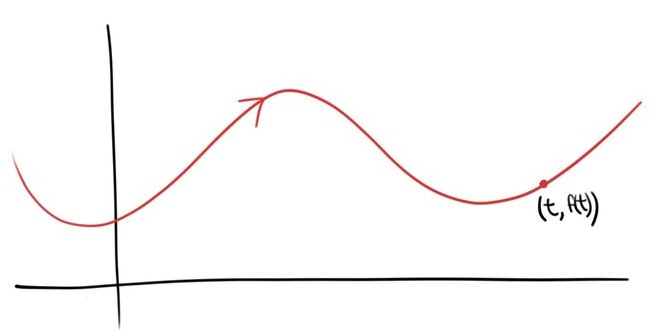
\includegraphics[width=0.6\textwidth]{C:/Users/Nacho/Documents/Latex/Facultad/GeometriaProyectiva/GeoProyectiva/graficofuncion.jpg}
	\caption{El gráfico de una función $f:I\to\RR$.}
	\label{fig:graficofuncion}
\end{figure}
\item Podemos dar curvas planas en términos de \textbf{coordenadas polares}. Es decir, parametrizamos $\alpha:I\to\RR^n$, $\alpha(\theta)=(\rho(\theta)\cos(\theta),\rho(\theta)\sen(\theta))$, donde $\rho:I\to\RR_{>0}$ es una función de clase $\mathscr{C}^k$. Veamos que $\alpha$ parametriza a una curva regular. En efecto, $\alpha'(\theta) = \rho'(\theta)(\cos(\theta),\sen(\theta)) + \rho(\theta)(-\sen(\theta),\cos(\theta))$. Como $(\cos(\theta),\sen(\theta))$ y $(-\sen(\theta),\cos(\theta))$ son vectores unitarios ortogonales, por Pitágoras tenemos que $\norm{\alpha'(\theta)}^2 = \abs{\rho(\theta)}^2 + \abs{\rho'(\theta)}^2$. Eso implica que $\alpha'$ sólo se anula si $\rho(\theta)=\rho'(\theta)=0$ y eso no puede pasar pues $\rho$ siempre es positiva.
\item La parametrización es muy importante. El conjunto $\mathscr{C}=\{(x,y)\in\RR^2:x=y\}$ admite muchas parametrizaciones. Por ejemplo, $\alpha,\beta:\RR\to\RR^2$, $\alpha(t)=(t,t)$ y $\beta(t)=(t^3,t^3)$. La primera es regular pues $\alpha'(t)=(1,1)$ mientras que la segunda no, pues $\beta'(t)=(3t^2,3t^2)$ es singular en $t=0$.
\item Consideremos la curva parametrizada por $\alpha:\RR\to\RR^2$, $\alpha(t)=(t^2,t^3)$. Esta curva no es regular, pues $\alpha'(t)=(2t,3t^2)$ es singular en $t=0$. Gráficamente, se puede ver que en el punto $t=0$ la curva no admite una recta tangente.
\begin{figure}[h]
	\centering
		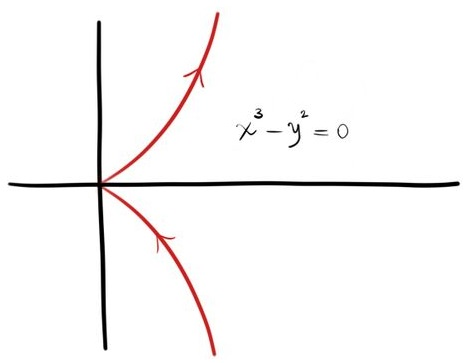
\includegraphics[width=0.4\textwidth]{C:/Users/Nacho/Documents/Latex/Facultad/GeometriaProyectiva/GeoProyectiva/curvacusp.jpg}
	\caption{La imagen de la curva $x^3 - y^2 = 0$, con su singularidad en $(0,0)$.}
	\label{fig:curvacusp}
\end{figure}
\end{itemize}
\end{ex}

\begin{lem}
Sea $\sigma:(a,b)\to\RR^n$ una curva regular. Si $c\in (a,b)$, entonces existe $\eps>0$ tal que $(c-\eps,c+\eps)\subseteq (a,b)$ y $\left.\sigma\right|_{(c-\eps,c+\eps)}$ es inyectiva. Es decir, toda curva es localmente inyectiva.
\begin{proof}
Supongamos que el enunciado es falso. Es decir, existe $c\in (a,b)$ tal que para todo $m\in\NN$, en cada intervalo $\left(c-\dfrac{1}{m},c+\dfrac{1}{m}\right)$ existen $x_m<y_m$ de tal modo que $\sigma(x_m)=\sigma(y_m)$ y además $\displaystyle\lim_{m\to\infty}x_m = c = \displaystyle\lim_{m\to \infty}y_m$. Tomemos $i\in\{1,\ldots , n\}$. Como $\sigma_i(x_m)=\sigma_i(y_m)$, por el Teorema del Valor Medio, existe $\xi_m^{(i)}\in (x_m,y_m)$ tal que $\sigma_i'(\xi_m^{(i)})=0$. Claramente, $\lim_{m\to\infty}\xi_m^{(i)}=c$. Por lo tanto (asumiendo una regularidad de clase $\mathscr{C}^1$ al menos) tendremos que $0=\displaystyle\lim_{m\to\infty}\sigma_i'(\xi_m^{(i)})=\sigma_i'(c)$. Por lo tanto, $\sigma'(c)=0$, contradiciendo que $\sigma$ es una curva regular.
\end{proof}
\end{lem}

\begin{cor}
Si $\sigma:(a,b)\to\RR^n$ es una curva regular, entonces todo punto de $\RR^n$ tiene un número finito de preimágenes en cada intervalo cerrado y acotado $[c,d]\subseteq (a,b)$.
\begin{proof}
En virtud del lema anterior, para cada $x\in [c,d]$ existe $\eps_x>0$ tal que $\left.\sigma\right|_{(x-\eps_x,x+\eps_x)}$ es inyectiva. El conjunto $\{(x-\eps_x,x+\eps_x) : x\in [c,d]\}$ es claramente un cubrimiento por abiertos de $[c,d]$, y por la compacidad, deben existir $x_1,\ldots , x_\ell$ de modo tal que $[c,d]\subseteq\displaystyle\bigcup_{i=1}^{\ell} (x_i-\eps_{x_i},x_i+\eps_{x_i})$. Por lo tanto, si $v\in\RR^n$, se sigue que: $$\sigma^{-1}(v)\cap [c,d] \subseteq \displaystyle\bigcup_{i=1}^\ell (x_i-\eps_{x_i},x_i+\eps_{x_i})\cap \sigma^{-1}(v)$$ Como la restricción de $\sigma$ a cada intervalo $(x_i-\eps_{x_i},x_i+\eps_{x_i})$ es inyectiva, esa unión tiene a lo sumo $\ell$ elementos. Y estamos.
\end{proof}
\end{cor}

\begin{ex}
Por lo general es falso que la fibra sea finita si no nos restringimos a un compacto. Por ejemplo, $\sigma:\RR\to\RR^2$ dada por $\sigma(t)=(\cos t,\sen t)$ tiene fibra $\sigma^{-1}((x_0,y_0)) = \{t_0 + 2k\pi : (\cos(t_0),\sen(t_0))=(x_0,y_0), k\in\ZZ\}$, que es infinita para cualquier punto $(x_0,y_0)$ en la circunferencia unitaria. Esto nos muestra que una curva posee más información que solamente su traza. Además, tenemos varias parametrizaciones distintas que describen una misma traza, como por ejemplo $\sigma_1:(0,2\pi)\to \RR^2$ dada por $\sigma_1(t)=(\cos(t),\sen(t))$ o $\sigma_2:(0,1)\to \RR^2$ dada por $\sigma_2(t)=(\cos(2\pi t),\sen(2\pi t))$.
\begin{figure}[h]
	\centering
		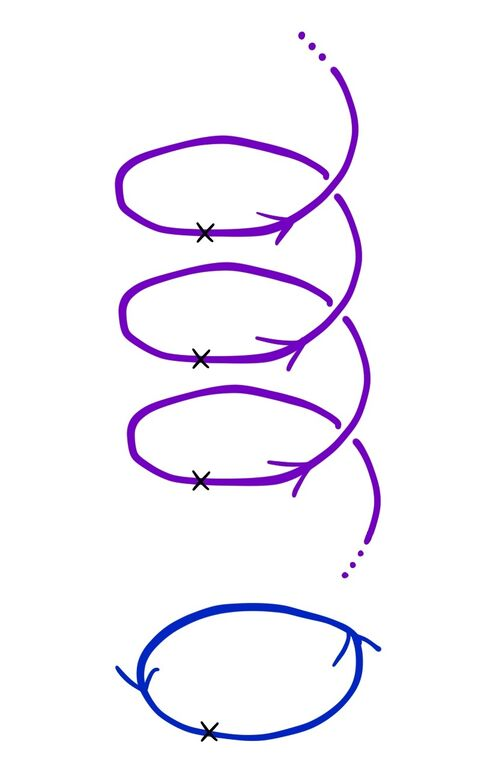
\includegraphics[width=0.25\textwidth]{C:/Users/Nacho/Documents/Latex/Facultad/GeometriaProyectiva/GeoProyectiva/revestimientos1.jpg}
	\caption{Una parametrización de $\mathrm{S}^1$ cuya fibra no es finita.}
	\label{fig:revestimientos1}
\end{figure}
\end{ex}

\begin{defn}
Una \textbf{reparametrización} es una función $u:(a,b)\to (c,d)$ biyectiva, diferenciable y con inversa diferenciable.
\end{defn}

\begin{defn}
Si $\sigma:(a,b)\to\RR^n$ es una curva regular y $u:(c,d)\to (a,b)$ es una reparametrización, entonces $\sigma\circ u:(c,d)\to\RR^n$ es una curva regular y se dice que $\sigma\circ u$ es una \textbf{reparametrización} de $\sigma$. Decimos $u$ que es una \textbf{reparametrización directa} si $u'(t)>0 \;\forall t\in (c,d)$.
\end{defn}

Como ya vimos, una curva posee más información que meramente su traza. Vamos a estudiar propiedades de las curvas que sean invariantes por movimientos rígidos y por reparametrización.

\section{Invariantes}

\begin{defn}
Sea $\mathscr{C}(n)$ el conjunto de pares $(\sigma,s_0)$ con $\sigma_I\to\RR^n$ una curva regular y $s_0\in I$. Un miembro del conjunto $\mathscr{C}(n)$ se llama un \textbf{elemento de curva}.
\end{defn}

\begin{defn}
Un \textbf{invariante escalar} es una función $V:\mathscr{C}(n)\to\RR$ que permanece invariante bajo movimientos rígidos y reparametrizaciones directas. Es decir, tal que $V(f\circ\sigma,s_0) = V(\sigma,s_0)$ para todo $f\in\Iso^+(n)$ y además $V(\sigma\circ u,u^{-1}(s_0)) = V(\sigma,s_0)$ para toda reparametrización directa $u:(a,b)\to \mathrm{Dom}\sigma$.
\end{defn}

\begin{defn}
Un \textbf{invariante vectorial} es una función $V:\mathscr{C}(n)\to\RR^n$ que cumple que $V(f\circ\sigma,s_0)=A_f V(\sigma,s_0)$ para todo $f\in\Iso^+(n)$ y $V(\sigma\circ u,u^{-1}(s_0)) = V(\sigma,s_0)$ para toda reparametrización directa $u:(a,b)\to\mathrm{Dom}\sigma$.
\end{defn}

\begin{comm}
Dado un grupo $G$ y dos conjuntos $X,Y$ provistos de acciones $G\acts X$, $G\acts Y$, una función $f:X\to Y$ se dice \textbf{equivariante} si $f(g\cdot x)=g\cdot f(x)$ para todos $x\in X,g\in G$. Es decir, el siguiente diagrama conmuta:

\begin{center}
\begin{tikzcd}
X \arrow[]{r}[font=\normalsize]{\cdot g}\arrow[]{d}[font=\normalsize, left]{f} & X\arrow[]{d}[font=\normalsize, right]{f} \\
Y \arrow[]{r}[font=\normalsize]{\cdot g} & Y
\end{tikzcd}
\end{center}

Si consideramos a $\Iso^+(n)$ actuando en $\mathscr{C}(n)$ vía $f\cdot (\sigma,s_0) = (f\circ\sigma,s_0)$ y a $\Iso^+(n)$ actuando en $\RR^n$ por $f\cdot x = A_f x$, entonces un invariante vectorial $V:\mathscr{C}(n)\to\RR^n$ es simplemente un morfismo equivariante respecto de estas acciones que es invariante bajo reparametrizaciones directas.
\end{comm}

\begin{defn}
Dos elementos de curva $(\sigma,s_0),(\tau,t_0)$ definen el mismo \textbf{germen} si existe $I\subseteq \mathrm{Dom}\sigma\cap\mathrm{Dom}\tau$ tal que $s_0=t_0\in I$ y además $\left.\sigma\right|_{I} = \left.\tau\right|_{I}$. Lo notaremos $(\sigma,s_0)\sim (\tau,t_0)$. Claramente $\sim$ es una relación de equivalencia y llamaremos al conjunto de clases de equivalencia (es decir, $\mathscr{C}(n)/\sim$) el conjunto de \textbf{gérmenes}. Si $x\in\RR^n$, denotamos por $\mathcal{O}_x$ al conjunto de gérmenes en $x$, es decir, las clases de equivalencia $[(\sigma,s_0)]$ tales que $\sigma(s_0)=x$ (notar que esto no depende del representante $(\sigma,s_0)$). Los gérmenes nos proveerán del contexto adecuado para estudiar propiedades locales. 
\begin{figure}[h]
	\centering
		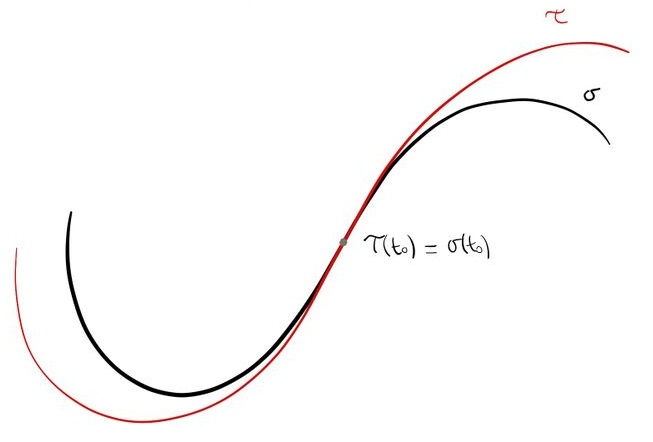
\includegraphics[width=0.5\textwidth]{C:/Users/Nacho/Documents/Latex/Facultad/GeometriaProyectiva/GeoProyectiva/curvasgermen.jpg}
	\caption{Dos curvas en un mismo germen.}
	\label{fig:curvasgermen}
\end{figure}
\end{defn}

\begin{obs}\label{obs::germenderivadas}
Sean $(\sigma,s_0)$ y $(\tau,t_0)$ dos elementos de un mismo germen. Entonces, $\sigma'(s_0)=\tau'(t_0)$. En efecto, notemos que como están en el mismo germen existe un intervalo $I$ tal que $s_0=t_0$ y $\left.\sigma\right|_{I}=\left.\tau\right|_{I}$, y así el cociente incremental coincide en un entorno de $s_0=t_0$. Tomando límite se sigue lo deseado.
\end{obs}

\begin{defn}
Un invariante $V$ (escalar o vectorial) se dice \textbf{local} si para todo par de elementos de curva $(\sigma,s_0),(\tau,t_0)\in\mathscr{C}(n)$ vale que: $$(\sigma,s_0)\sim(\tau,t_0) \Longrightarrow V(\sigma,s_0) = V(\tau,t_0)$$ Es decir, es un invariante que es constante en los gérmenes.
\end{defn}

\begin{defn}
Un invariante $V$ (escalar o vectorial) se dice \textbf{diferencial} de orden menor o igual que $d$ si existe una función $W:(\RR^n)^{d+1}\to \RR$ ó $\RR^n$ (según si $V$ es escalar o vectorial respectivamente) tal que para todo elemento de curva $(\sigma,s_0)\in\mathscr{C}(n)$ se tiene que: $$V(\sigma,s_0)=W(\sigma(s_0),\sigma'(s_0),\ldots ,\sigma^{(d)}(s_0))$$ Decimos que un invariante diferencial es de orden $d$ si es de orden menor o igual que $d$ pero no de orden menor o igual que $d-1$.
\end{defn}

\begin{obs} Por la Observación ~\ref{obs::germenderivadas}, es claro que todo invariante diferencial es local.
\end{obs}

Nuestro objetivo ahora será tratar de caracterizar a los invariantes diferenciales. Empecemos con los invariantes de orden bajo. 

\begin{prop}
Sea $V$ un invariante diferencial escalar de orden $0$. Entonces $V$ es constante.
\begin{proof}
Sea $V:\mathscr{C}(n)\to \RR$ un invariante escalar diferencial de orden $0$. Luego, existe $W:\RR^n\to\RR$ tal que $V(\sigma,s_0)=W(\sigma(s_0))$. Notemos que: $$W(f(\sigma(s_0))) = V(f\circ\sigma,s_0)=V(\sigma,s_0)=W(\sigma(s_0))$$ para todo $(\sigma,s_0)\in\mathscr{C}(n)$, $f\in\Iso^+(n)$. Esto implica que $W(f(v))=W(v)$ para todo $v\in\RR^n$, $f\in\Iso^+(n)$. Ahora, si $w\in\RR^n$ es arbitrario, sea $f(x)=x+(w-v)$. Claramente se cumple que $f\in\Iso^+(n)$, $f(v)=w$ y así $W(w)=W(f(v))=W(v)$. Es decir, $W$ es constante. Como queríamos.
\end{proof}
\end{prop}

\begin{prop}
Sea $V$ un invariante diferencial vectorial de orden $0$. Entonces $V\equiv 0$.
\begin{proof}
Sea $V:\mathscr{C}(n)\to\RR^n$ un invariante vectorial diferencial de orden $0$. Luego, existe $W:\RR^n\to\RR^n$ tal que $V(\sigma,s_0)=W(\sigma(s_0))$. Notemos que: $$W(f(\sigma(s_0))) = V(f\circ\sigma,s_0)=A_f V(\sigma,s_0) = A_f W(\sigma,s_0)$$ para todo $(\sigma,s_0)\in\mathscr{C}(n)$, $f\in\Iso^+(n)$. Esto implica que $W(f(v))=A_f W(v)$ para todo $v\in\RR^n$, $f\in\Iso^+(n)$. Ahora, sea $h:\RR^n\to\RR^n$ la traslación $h(x)=x-v$. Claramente $A_h=I$ y así $W(v)=W(0)$. Es decir, $W$ es constante. Pero más aún, sea $g:\RR^n\to\RR^n$ la transformación $g(x)=Ax$ con $A\in\mathrm{SO}(n)$. Por lo tanto, $AW(0)=W(0)$ para toda $A\in\mathrm{SO}(n)$. Esto implica que $W(0)=0$ pues si $W(0)\neq 0$, completando a una base ortogonal y tomando $A$ como la reflexión en $W(0)$ y algún otro vector de la base (para que el determinante sea $1$), obtenemos que $-W(0) = AW(0) = W(0)$. Y estamos.
\end{proof}
\end{prop}

\begin{prop}
Sea $V$ un invariante diferencial escalar de orden $1$. Entonces $V$ es constante.
\begin{proof}
Sea $W:(\RR^n)^2\to\RR$ con $V(\sigma,s_0)=W(\sigma(s_0),\sigma'(s_0))$. Sea $(\sigma,s_0)\in\mathscr{C}(n)$ y consideremos $f_1:\RR^n\to\RR^n$, $f_1(x)=x-\sigma(s_0)$. Notemos que por regla de la cadena $(f\circ\sigma)'(s_0) = \sigma'(s_0)$ y así $V(\sigma,s_0)=V(f\circ\sigma,s_0)=W(0,\sigma'(s_0))$. Entonces, si defino $W_1:\RR^n\to\RR$ por $W_1(v)=W(0,v)$, la función $V$ queda determinada totalmente por $W_1$.
Supongamos sin pérdida de la generalidad que $\sigma(s_0)=0$, y sea $A\in\mathrm{SO}(n)$. Consideremos $f_2:\RR^n\to\RR^n$ la isometría dada por $f_2(x)=Ax$. Entonces, es claro que: $$W_1(A\sigma'(s_0)) = W(0,A\sigma'(s_0)) = V(f_2\circ\sigma,s_0) = V(\sigma,s_0)=W(0,\sigma'(s_0))=W_1(\sigma'(s_0))$$
Es decir, para todos $(\sigma,s_0)\in\mathscr{C}(n)$ tal que $\sigma(s_0)=0$ y $A\in\mathrm{SO}(n)$, tenemos que $W_1(A\sigma'(s_0))=W_1(\sigma'(s_0))$. Esto implica que para todo $v\in\RR^n\smallsetminus\{0\}$ y $A\in\mathrm{SO}(n)$, tenemos que $W_1(v)=W_1(Av)$. Ahora bien, el conjunto $\{Av:A\in\mathrm{SO}(n)\}$ es simplemente la esfera de centro $0$ y radio $\norm{v}$. Esto quiere decir que $W_1$ es una función radial. O sea, existe $W_2:\RR_{>0}\to\RR$ tal que $W_1(v)=W_2(\norm{v})$. Por lo tanto, $V(\sigma,s_0)=W_2(\norm{\sigma'(s_0)})$. Consideremos ahora una reparametrización directa $u:(c,d)\to\mathrm{Dom}\sigma$. Entonces: $$W_2(\norm{\sigma'(s_0)}) = V(\sigma,s_0)=V(\sigma\circ u,u^{-1}(s_0)) = W_2\left(\abs{u'(u^{-1}(s_0))}\norm{\sigma'(s_0)}\right)$$ Luego, para todo $v\in\RR^n\smallsetminus\{0\}$ y $u:(c,d)\to\mathrm{Dom}\sigma$ reparametrización directa, tenemos que $W_2(\norm{v})=W_2(\abs{u'(u^{-1}(s_0))}\norm{v})$. Tomando la reparametrización $u(t)=\lambda t$, se sigue que $W_2(\norm{v})=W_2(\lambda\norm{v})$ para todo $v\in\RR^n\smallsetminus\{0\}$, $\lambda>0$. Tomando $v$ de norma $1$ y $\lambda>0$ arbitrario, resulta que $W_2$ es constante y así $V$ debe serlo. Como queríamos probar.
\end{proof}
\end{prop}

Hasta ahora todos los invariantes son triviales. Los invariantes vectoriales de orden $1$ son los primeros que son interesantes, pero para aliviar la notación, primero consideremos la siguiente definición:

\begin{defn}
Sea $(\sigma,s_0)\in\mathscr{C}(n)$ un elemento de curva. Se define el \textbf{vector tangente} a $\sigma$ en $s_0$ como $\T(\sigma,s_0)=\dfrac{\sigma'(s_0)}{\norm{\sigma'(s_0)}}$. Cuando $n=2$, podemos definir el \textbf{vector normal} a $\sigma$ en $s_0$ como $\N(\sigma,s_0) = (-\T(\sigma,s_0)_2, \T(\sigma,s_0)_1)$ es el único vector unitario que completa a una base a $\T(\sigma,s_0)$ de manera tal que "`preserve la orientación"' (es decir, que el determinante de la matriz cuyas columnas son $\T(\sigma,s_0)$ y $\N(\sigma,s_0)$ sea $1$).
\end{defn}

\begin{prop}
Sea $V$ un invariante diferencial vectorial de orden $1$. Entonces, si $n\geq 3$, $V(\sigma,s_0) = \lambda\T(s_0)$ con $\lambda\in\RR$, mientras que si $n=2$, $V(\sigma,s_0)=a\T(\sigma,s_0)+b\N(\sigma,s_0)$ con $a,b\in\RR$.
\begin{proof}
Sea $W:(\RR^n)^2\to\RR^n$ tal que $V(\sigma,s_0)=W(\sigma(s_0),\sigma'(s_0))$. Consideremos $g:\RR^n\to\RR^n$ dada por $f(x)=A(x-\sigma(s_0))$ donde $A\in\mathrm{SO}(n)$. Por lo tanto, se tiene que $AV(\sigma,s_0)=V(g\circ\sigma,s_0) =W(0,A\sigma'(s_0))$. Consideremos $A$ una rotación que lleva $\sigma'(s_0)$ a $\norm{\sigma'(s_0)}e_1$ (equivalentemente, $\T(\sigma,s_0)$ a $e_1$). Esta rotación en $n=2$ queda unívocamente determinada como la matriz cuya inversa tiene por columnas a $\T(\sigma,s_0)$ y $\N(\sigma,s_0)$, mientras que en $n\geq 3$ tenemos mayor libertad y no queda unívocamente determinada. 
Por lo tanto, se sigue que $V(\sigma,s_0) = A^{-1}W(0,\norm{\sigma'(s_0)}e_1)$. Sea $u:\mathrm{Dom}\sigma\to\mathrm{Dom}\sigma$ la reparametrización directa dada por $u(t)=s_0+\dfrac{t}{\norm{\sigma'(s_0)}}$. Como $V$ es un invariante: $$V(\sigma,s_0)=V(\sigma\circ u,0)=W(0,\sigma'(s_0)u'(0)) = W(0,\T(\sigma,s_0))$$ Si tengo entonces $(\sigma,s_0)$ un elemento de curva tal que $\sigma(s_0)=0$ y $\sigma'(s_0)=e_1$, entonces $V(\sigma,s_0)=W(0,\T(\sigma,s_0)) = W(0,e_1)$. 

\begin{figure}[h]
	\centering
		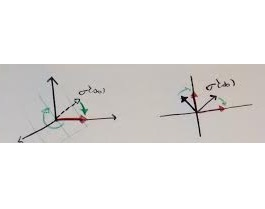
\includegraphics[width=0.4\textwidth]{C:/Users/Nacho/Documents/Latex/Facultad/GeometriaProyectiva/GeoProyectiva/rotacionlibre.jpg}
	\caption{Una rotación que lleva a $\sigma'(s_0)$ al eje $e_1$. En el caso plano queda determinada.}
	\label{fig:rotacionlibre}
\end{figure}

Supongamos que $n\geq 3$, y $M\in\mathrm{SO}(n)$ es alguna rotación que deja fijo a $e_1$. Entonces: $$W(0,e_1)=W(0,Me_1)=V(M\circ\sigma,s_0)=MV(\sigma,s_0)=MW(0,e_1)$$ Esto quiere decir que $W(0,e_1)$ queda fijo por cualquier rotación que deja fijo a $e_1$. Eso implica que $W(0,e_1)=\lambda e_1$, pues en el complemento ortogonal de $e_1$ podemos definir la transformación como querramos (siempre y cuando $Me_i\in\langle e_1\rangle^{\perp}$). Por lo tanto, si $n\geq 3$ tendremos que $V(\sigma,s_0)=A^{-1}W(0,e_1)=\lambda A^{-1}e_1 = \lambda \T(\sigma,s_0)$. 

\begin{figure}[h]
	\centering
		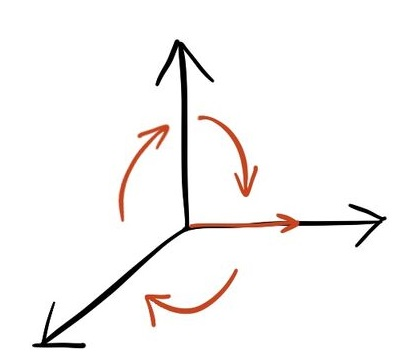
\includegraphics[width=0.3\textwidth]{C:/Users/Nacho/Documents/Latex/Facultad/GeometriaProyectiva/GeoProyectiva/rotacionfijae1.jpg}
	\caption{Una rotación en $\RR^3$ que deja fijo al eje $e_1$.}
	\label{fig:rotacionfijae1}
\end{figure}

Para $n=2$, sabemos que $A^{-1}$ queda unívocamente determinada como la matriz cuyas columnas son $\T(\sigma,s_0)$ y $\N(\sigma,s_0)$ y si $W(0,e_1)=ae_1 + be_2$, obtenemos que: $$V(\sigma,s_0)=A^{-1}W(0,e_1) = a\T(\sigma,s_0)+b\N(\sigma,s_0)$$ que es fácil comprobar que es un invariante (pues el par $\{\T(\sigma,s_0),\N(\sigma,s_0)\}$ forma siempre una base ortonormal con determinante $1$). Y estamos.
\end{proof}
\end{prop}

Por último, vamos a caracterizar los invariantes diferenciales escalares de orden $2$. Para ello, antes consideremos la siguiente definición:

\begin{defn}
Sea $(\sigma,s_0)\in\mathscr{C}(n)$. Se define la \textbf{curvatura} de $\sigma$ en $s_0$ como: $$\kappa(\sigma,s_0)=\dfrac{\sqrt{\norm{\sigma'(s_0)}^2\norm{\sigma''(s_0)}^2 - \langle\sigma'(s_0),\sigma''(s_0)\rangle^2}}{\norm{\sigma'(s_0)}^3}$$
\end{defn}

Notemos que la curvatura $\kappa(\sigma,s_0)$ es un invariante diferencial escalar de orden $2$. En efecto, si $f:\RR^n\to\RR^n$, $f\in\Iso^+(n)$, entonces tenemos que $(f\circ\sigma)'(s_0)=A_f\sigma'(s_0)$ y $(f\circ\sigma)''(s_0)=A_f\sigma''(s_0)$, y reemplazando en la fórmula de la curvatura (y notando que $A_f\in\mathrm{SO}(n)$ y así preserva ángulos y distancias), es claro que $\kappa(f\circ\sigma,s_0)=\kappa(\sigma,s_0)$. Por otra parte, si $u:(c,d)\to\mathrm{Dom}\sigma$ es una reparametrización directa, por la regla de la cadena es fácil ver que se tiene $(\sigma\circ u)'(u^{-1}(s_0)) = \sigma'(s_0)u'(u^{-1}(s_0))$ y también tenemos $(\sigma\circ u)''(u^{-1}(s_0)) = \sigma''(s_0) u'(u^{-1}(s_0))^2 + \sigma'(s_0)u''(u^{-1}(s_0))$. Es fácil comprobar, usando esto, que $\kappa(\sigma\circ u,u^{-1}(s_0)) = \kappa(\sigma,s_0)$. Notemos también que si $\varphi:\RR_{>0}\to\RR$ es una función cualquiera, entonces $\varphi(\kappa(\sigma,s_0))$ también es un invariante diferencial escalar de orden $2$. Veamos que vale la recíproca:

\begin{prop}
Sea $V$ un invariante diferencial escalar de orden $2$. Entonces, existe una función $\varphi:\RR_{>0}\to\RR$ tal que $V(\sigma,s_0)=\varphi(\kappa(\sigma,s_0))$.
\begin{proof}
Consideremos $A\in\mathrm{SO}(n)$ tal que $A\sigma'(s_0)=\norm{\sigma'(s_0)}e_1$, la traslación ${f:\RR^n\to\RR^n}$ dada por $f(x)=A(x-\sigma(s_0))$ y la reparametrización $u(s)=s_0+\dfrac{s-s_0}{\norm{\sigma'(s_0)}}$. Es claro que $u^{-1}(s_0)=s_0$. Considero entonces $\gamma = f\circ\sigma\circ u$. Como $V$ es un invariante, tenemos que $V(\gamma,s_0)=V(f\circ\sigma\circ u,s_0)=V(\sigma\circ u,s_0)=V(\sigma,s_0)$. Pero tenemos que $\gamma(s_0)=0$, $\gamma'(s_0)=e_1$ y así $V(\gamma,s_0)=W(0,e_1,\gamma''(s_0))$, donde $W:(\RR^n)^3\to\RR$ es la función tal que $V(\sigma,s_0)=W(\sigma(s_0),\sigma'(s_0),\sigma''(s_0))$. 

Sea $M\in\mathrm{SO}(n)$ una rotación con eje $e_1$ (es decir, $Me_1=e_1$). Entonces, si $g:\RR^n\to\RR^n$, $g(x)=Mx$, se cumple que $W(0,e_1,M\gamma''(s_0))=V(g\circ\gamma,s_0)=V(\gamma,s_0)=W(0,e_1,\gamma''(s_0))$. Por otra parte, supongamos que $u:(a,b)\to\mathrm{Dom}\sigma$ es una reparametrización directa tal que $s_0\in (a,b)$, $u(s_0)=s_0$ y $u'(s_0)=1$. Entonces, por la regla de la cadena, tenemos que $W(0,e_1,u''(s_0)\gamma'(s_0)+\gamma''(s_0)) = V(\gamma\circ u,s_0)=V(\gamma,s_0)=W(0,e_1,\gamma''(s_0))$. En resumen, si definimos $\Phi(v)=W(0,e_1,v)$, tendremos que $\Phi(A\gamma''(s_0))=\Phi(\gamma''(s_0))$ para toda ${M\in\mathrm{SO}(n)}$ tal que $Me_1=e_1$, y tendremos que $\Phi(u''(s_0)e_1+\gamma''(s_0))=\Phi(\gamma''(s_0))$ para toda reparametrización $u$ tal que $u(s_0)=s_0$ y $u'(s_0)=1$.

Si consideramos la curva $\gamma(s)=(s-s_0)e_1 + \dfrac{(s-s_0)^2}{2}v$, con $v\in\RR^n$, se tiene que $\gamma'(s_0)=e_1\neq 0$ y así define una curva regular en un entorno de $s_0$. Como los invariantes están definidos a menos del germen, podemos mirar $V(\gamma,s_0)$. Esta curva $\gamma$ cumple que $\gamma(s_0)=0$, $\gamma'(s_0)=e_1$ y $\gamma''(s_0)=v$. Por lo tanto, $\Phi(v)=\Phi(Mv)$ para toda $M\in\mathrm{SO}(n)$ tal que $Me_1=e_1$. Ahora, consideremos la reparametrización $u_\lambda(s)=s_0 + \lambda\dfrac{(s-s_0)^2}{2}$, definida en un entorno de $s_0$. Luego, tenemos que $\Phi(\lambda e_1 + v)=\Phi(v)$. Es decir, $\Phi$ es constante sobre cilindros con eje $e_1$. Por lo tanto, para definir $\Phi(v)$ sólo nos importa la norma de su proyección ortogonal sobre $\langle e_1\rangle^{\perp}$. Esto implica que existe $\varphi:\RR_{>0}\to\RR$ tal que $\Phi(v)=\varphi(\norm{v-\pint{v,e_1}e_1})$ para todo $v\in\RR^n$.

Ahora bien, juntando todo lo que hicimos, tenemos la siguiente fórmula: $$V(\sigma,s_0)=W(0,e_1,\gamma''(s_0))=\Phi(\gamma''(s_0))=\varphi(\norm{\gamma''(s_0)+\pint{\gamma''(s_0),e_1}e_1})$$ donde $\gamma(s)=f\circ\sigma\circ u(s)$ como en el primer párrafo. Es fácil comprobar, por la regla de la cadena, que $\gamma''(s_0)=A\dfrac{\sigma''(s_0)}{\norm{\sigma'(s_0)}^2}$. Además, notemos que como $A\sigma'(s_0) = \norm{\sigma'(s_0)}e_1$, se tiene que $A\dfrac{\sigma'(s_0)}{\norm{\sigma'(s_0)}} = e_1$. Estamos en condiciones de calcular la norma de la proyección ortogonal de $\gamma''(s_0)$. Simplemente es escribir todo y usar que $A\in\mathrm{SO}(n)$ preserva ángulos y distancias. En efecto: \begin{align*}\norm{\gamma''(s_0)+\pint{\gamma''(s_0),e_1}e_1} &= \norm{A\dfrac{\sigma''(s_0)}{\norm{\sigma'(s_0)}^2} - \pint{A\dfrac{\sigma''(s_0)}{\norm{\sigma'(s_0)}^2},A\dfrac{\sigma'(s_0)}{\norm{\sigma'(s_0)}}}A\dfrac{\sigma'(s_0)}{\norm{\sigma'(s_0)}}} \\ &= \norm{A\left(\dfrac{\sigma''(s_0)}{\norm{\sigma'(s_0)}^2} - \pint{A\dfrac{\sigma''(s_0)}{\norm{\sigma'(s_0)}^2},A\dfrac{\sigma'(s_0)}{\norm{\sigma'(s_0)}}}\dfrac{\sigma'(s_0)}{\norm{\sigma'(s_0)}}\right)}\\&= \norm{\dfrac{\sigma''(s_0)}{\norm{\sigma'(s_0)}^2} - \pint{\dfrac{\sigma''(s_0)}{\norm{\sigma'(s_0)}^2},\dfrac{\sigma'(s_0)}{\norm{\sigma'(s_0)}}}\dfrac{\sigma'(s_0)}{\norm{\sigma'(s_0)}}} \\ &= \dfrac{\norm{\sigma''(s_0)\norm{\sigma'(s_0)}^2 - \pint{\sigma'(s_0),\sigma''(s_0)}\sigma'(s_0)}}{\norm{\sigma'(s_0)}^4}\\&=\dfrac{\sqrt{\norm{\sigma''(s_0)^2}\norm{\sigma'(s_0)}^4 -\norm{\sigma'(s_0)}^2\pint{\sigma'(s_0),\sigma''(s_0)}^2}}{\norm{\sigma'(s_0)}^4} \\ &= \dfrac{\sqrt{\norm{\sigma'(s_0)}^2\norm{\sigma''(s_0)}^2 - \pint{\sigma'(s_0),\sigma''(s_0)}^2}}{\norm{\sigma'(s_0)}^3}\end{align*}Es decir, hemos probado que $\norm{\gamma''(s_0)+\pint{\gamma''(s_0),e_1}e_1} = \kappa(\sigma,s_0)$. Como ya habíamos visto que $V(\sigma,s_0)=\varphi(\norm{\gamma''(s_0)+\pint{\gamma''(s_0),e_1}e_1})$, esto nos dice que $V(\sigma,s_0)=\varphi(\kappa(\sigma,s_0))$. Esto concluye la demostración.
\end{proof}
\end{prop}

Consideremos por un momento invariantes escalares de curvas planas. Es decir, invariantes $V:\mathscr{C}(2)\to\RR$. Sea $(\sigma,s_0)\in\mathscr{C}(2)$, con $\sigma:(a,b)\to\RR^n$. Podemos considerar $V_\sigma:(a,b)\to\RR$ definida por $V_\sigma(s)=V(\sigma,s)$. Decimos que $V$ es un invariante \textbf{diferenciable} si existe la derivada $\left.\dfrac{\mathrm{d}}{\mathrm{ds}}\right\rvert_{s=s_0} V_\sigma(s)$. Claramente, la derivada está bien definida en el germen (pues si $(\sigma,s_0)\sim(\tau,t_0)$ entonces $\sigma$ y $\tau$ coincidirán en un entorno de $s_0=t_0$ y así $V_\sigma$ y $V_\tau$ también). Consideremos entonces la asignación $U:\mathscr{C}(2)\to\RR$ dada por $U(\sigma,s_0)=\left.\dfrac{\mathrm{d}}{\mathrm{ds}}\right\rvert_{s=s_0} V_\sigma(s)$. Usando que $V$ es invariante, es fácil ver que $U(f\circ\sigma,s_0)=U(\sigma,s_0)$ para $f\in\Iso^+(n)$. Ahora, si $u:(c,d)\to\mathrm{Dom}\sigma$ es una reparametrización, tenemos que: \begin{align*}U(\sigma\circ u,u^{-1}(s_0)) = \left.\dfrac{\mathrm{d}}{\mathrm{dt}}\right\rvert_{t=u^{-1}(s_0)} V(\sigma\circ u,t)&=\left.\dfrac{\mathrm{d}}{\mathrm{dt}}\right\rvert_{t=u^{-1}(s_0)} V(\sigma,u(t))\\ &= u'(u^{-1}(s_0)) \left.\dfrac{\mathrm{d}}{\mathrm{ds}}\right\rvert_{s=s_0} V(\sigma,s)\\ &= U(\sigma,s_0)u'(u^{-1}(s_0))\end{align*} Es decir, $U$ \textbf{no} es un invariante, pero casi. Simplemente consideremos: $$DV(\sigma,s_0) = \dfrac{1}{\norm{\sigma'(s_0)}^2}\left.\dfrac{\mathrm{d}}{\mathrm{ds}}\right\rvert_{s=s_0} V_\sigma(s)$$ Esto es un invariante pues $\norm{\sigma'(s_0)}$ permanece invariante bajo movimientos euclídeos y con reparametrizaciones también aparece un factor $u'(u^{-1}(s_0))$ que se cancela con el de $U$. Es decir, construimos un invariante $DV$ a partir de $V$. Si $V$ es un invariante diferencial de orden a lo sumo $d$, entonces $DV$ debería ser de orden a lo sumo $d+1$ (pues escribimos $V(\sigma,s_0)=W(\sigma(s_0),\ldots,\sigma^{(d)}(s_0))$ y derivamos usando la regla de la cadena, si asumimos alguna condición de regularidad en $W$).

Ahora bien, en $\mathscr{C}(2)$ nosotros conocemos dos invariantes: la tangente $\T$ y la normal $\N$. Notemos que como $\norm{\T(\sigma,s)}^2 = 1$ para todo $s$, derivando el producto interno se sigue que $2\pint{\T(\sigma,s_0),\left.\dfrac{\mathrm{d}}{\mathrm{ds}}\right\rvert_{s=s_0}\T(\sigma,s)} = 0$ para todo $s_0$. Esto implica que para cualquier $s_0$ tenemos que $\N(\sigma,s_0)$ es paralelo a $D\T(\sigma,s_0)=\left.\dfrac{\mathrm{d}}{\mathrm{ds}}\right\rvert_{s=s_0} \T(\sigma,s)$. Por lo tanto, debemos tener que $D\T(\sigma,s_0) = \pint{D\T(\sigma,s_0),\N(\sigma,s_0)}\N(\sigma,s_0)$. Pero notemos que $\pint{D\T(\sigma,s_0),\N(\sigma,s_0)}$ es un invariante diferencial escalar de orden menor o igual que $2$, y por ende debe ser de la forma $\varphi(\kappa(\sigma,s_0))$ para alguna $\varphi:\RR_{>0}\to\RR$. Es decir, para todo $(\sigma,s_0)\in\mathscr{C}(2)$ se tiene que $D\T(\sigma,s_0)=\varphi(\kappa(\sigma,s_0))\N(\sigma,s_0)$. Entonces, si consideramos las circunferencias $\sigma_r:\RR\to\RR^2$, $\sigma_r(t)=(r\cos t,r\sen t)$ para $r>0$, es fácil ver que $\kappa(\sigma_r,s)=\dfrac{1}{r}$ para todo $s\in\RR$. Además, como $\T(\sigma_r,s)=(-\sen s,\cos s)$, $\N(\sigma_r,s)=-(\cos s,\sen s)$, se sigue que $D\T(\sigma,s)=\dfrac{1}{\norm{\sigma''(s_0)}}(-\cos s,\sen s) = \dfrac{1}{r}(-\cos s,\sen s) = \dfrac{1}{r}\N(\sigma,s)$. Por lo tanto, tenemos que $\varphi\left(\dfrac{1}{r}\right)=\dfrac{1}{r}$ para todo $r>0$, que implica $\varphi(x)=x$. 

Hemos probado que $D\T(\sigma,s_0)=\kappa(\sigma,s_0)\N(\sigma,s_0)$. De manera análoga, podemos probar la relación $D\N(\sigma,s_0)=-k(\sigma,s_0)\T(\sigma,s_0)$. Ahora bien, la primera relación se puede escribir como $\T' = \norm{\sigma'}\kappa\N$, y como $\T = \dfrac{\sigma'}{\norm{\sigma'}}$, derivando podemos expresar a $\sigma''$ en términos de $\sigma',\T,\kappa$ y $\N$. Procediendo así sucesivamente, podemos expresar a todas las derivadas de orden superior en términos de estos elementos, y así los únicos invariantes diferenciales relevantes en el plano son $\T,\N$ y $\kappa$.

Queremos eliminar ahora un poco de la arbitrariedad de la elección de la parametrización de la curva. Si pensamos en la parametrización como la manera de recorrer la curva, inmediatamente tenemos una forma natural de recorrerla: a rapidez constante. Esta manera de recorrerla será la denominada \textbf{reparametrización por longitud de arco}. ¿Cómo podemos definir la longitud de una curva? Lo que sí sabemos medir son segmentos, entonces la idea intuitiva es aproximar la curva con muchos segmentos y sumar las longitudes de estos. Es decir, si tenemos una curva $\sigma:(a,b)\to\RR^n$ y nos quedamos con un segmento de curva $\sigma:[c,d]\to\RR^n$, tomamos una partición $P=\{c=p_0<p_1<\ldots <p_n=d\}$ del intervalo $[c,d]$ y miramos la suma de los segmentos entre $\sigma(p_{i-1})$ y $\sigma(p_i)$ para cada $1\leq i\leq n$. Es decir, $S_P(\sigma)=\displaystyle\sum_{i=1}^n \norm{\sigma(p_i)-\sigma(p_{i-1})}=\displaystyle\sum_{i=1}^n \norm{\sigma'(\xi_i)}\norm{p_i-p_{i-1}}$ donde $\xi_i\in [p_{i-1},p_i] =\{t\in [0,1] : tp_{i-1}+(1-t)p_i\}$, por el Teorema del Valor Medio. Pero esto es una suma de Riemann para la integral $\displaystyle\int_c^d \norm{\sigma'(\xi)}\diff\xi$. Esto motiva entonces la siguiente definición:

\begin{defn}
Sea $\sigma:(a,b)\to\RR^n$ una curva regular y $\sigma:[c,d]\to\RR^n$ un segmento de curva ($[c,d]\subseteq (a,b)$). La longitud de $\sigma$ entre $c$ y $d$ se define por: $$\mathrm{Long}(\sigma_{[c,d]}) = \int_c^d \norm{\sigma'(\xi)}\diff\xi$$
\end{defn}

Notemos que, simplemente por el Teorema de Cambio de Variables, es claro que la longitud de un segmento de curva es invariante por reparametrizaciones y movimientos rígidos. Si tenemos una curva $\sigma:(a,b)\to\RR^n$ y $t_0\in (a,b)$ fijo, definimos la función $v:(a,b)\to\RR$ por $v(t)=\displaystyle\int_{t_0}^t \norm{\sigma'(\xi)}\diff\xi$. Esta función $v$ claramente es diferenciable (es más, tiene la misma regularidad que $\sigma$) y tenemos que $v'(t)>0$ para todo $t\in (a,b)$. Por lo tanto, existe una función inversa $u:(c,d)\to (a,b)$ y la curva $\gamma=\sigma\circ u:(c,d)\to\RR^n$ es tal que $\norm{\sigma'(s)}=1$ para todo $s\in (c,d)$. Es decir, $\gamma$ es una reparametrización de $\sigma$ a velocidad constante, la \textbf{reparametrización por longitud de arco} que buscabamos.

Como herramienta teórica, la reparametrización por longitud de arco es muy útil, pero veremos que calcularla rápidamente se convierte en un problema dificil. En efecto, consideremos una elipse parametrizada por $\sigma:\RR\to\RR^2$, $\sigma(t)=(a\cos(\omega t),b\sen(\omega t))$. Entonces, $\sigma'(t)=(-a\omega\sen(\omega t),b\omega\cos(\omega t))$ y así $\norm{\sigma'(t)}=\omega \sqrt{a^2\sen^2(\omega t) + b^2\cos^2(\omega t)}$. Sin embargo, la integral $\displaystyle\int_0^t \omega\sqrt{a^2\sen^2(\omega \xi)+b^2\cos^2(\omega \xi)}\diff \xi$ es una \textbf{integral elíptica de primera especie}, a la que no podemos encontrarle una primitiva en términos de funciones elementales.

\section{Curvas Planas}

Si $\sigma:(a,b)\to\RR^2$ es una curva regular parametrizada por longitud de arco, su tangente en $s$ es simplemente $\T(s)=\sigma'(s)$. Por lo tanto, podemos expresar a la tangente como $\T(s)=(\cos\theta(s),\sen\theta(s))$ donde $\theta(s)$ representa el ángulo que forma $\T(s)$ con la horizontal. El cambio instantáneo del ángulo nos debería dar una noción de cómo se esta \textit{curvando} la curva. Pero notemos que $\T'(s)=\theta'(s)(-\sen\theta(s),\cos\theta(s))$, y así se sigue que $\norm{T'(s)}=\abs{\theta'(s)}$. Tiene sentido considerar entonces la siguiente definición:

\begin{figure}[h]
	\centering
		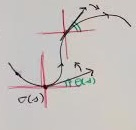
\includegraphics[width=0.4\textwidth]{C:/Users/Nacho/Documents/Latex/Facultad/GeometriaProyectiva/GeoProyectiva/curvaturaangular.jpg}
	\caption{La curvatura como el cambio angular.}
	\label{fig:curvaturaangular}
\end{figure}


\begin{defn}
Sea $\sigma:(a,b)\to\RR^n$ una curva regular parametrizada por longitud de arco. Se define la \textbf{curvatura} de $\sigma$ en $s$ por $\kappa(s)=\norm{\T'(s)}$.
\end{defn}

\begin{obs}
Veamos que los dos conceptos de curvatura que tenemos coinciden. Sabemos que $\kappa(\sigma,s_0)$ es invariante por reparametrización, así que si reparametrizamos a $\sigma$ por longitud de arco como $\gamma=\sigma\circ u$, tendremos que $\kappa(\sigma,s_0) = \kappa(\gamma,u^{-1}(s_0))$. Notando que $\norm{\gamma'(t)}=1$ y derivando el producto interno $\pint{\gamma'(t),\gamma'(t)}$ obtenemos que $\pint{\gamma'(t),\gamma''(t)}=0$ para todo $t$. Por lo tanto, reemplazando $t_0=u^{-1}(s_0)$, se tiene: $$\kappa(\sigma,s_0)=\kappa(\gamma,t_0)=\dfrac{\sqrt{\norm{\gamma'(t_0)}^2\norm{\gamma''(t_0)}^2 - \pint{\gamma'(t_0),\gamma''(t_0)}^2}}{\norm{\gamma'(t_0)}^3} = \norm{\gamma''(t_0)}=\kappa(t_0)$$ Tenemos así que $\kappa(\sigma,s_0)=\kappa(t_0)$. Es decir, el valor de ambas curvaturas en el punto $\sigma(s_0)=\gamma(t_0)$ de la curva es el mismo. Por lo tanto, tenemos una expresión para la curvatura que \textbf{no} depende de la reparametrización por longitud de arco, que en la práctica es dificil de calcular.
\end{obs}

\begin{ex}
Si $\sigma(s)=vs+w$ con $v,w\in\RR^n, \norm{v}=1$ parametriza una recta por longitud de arco, entonces $\T(s)=v$ y así $\T'(s)=0$, lo que implica que $\kappa(s)=0$. Es decir, una recta no está curvada. Por otra parte, si $\sigma(s)=\left(r\cos\dfrac{s}{r},r\sen\dfrac{s}{r}\right)$ parametriza a una circunferencia de centro $0$ y radio $r$ por longitud de arco, entonces $\T(s)=\left(-\sen\dfrac{s}{r},\cos\dfrac{s}{r}\right)$ y $\T'(s)=\dfrac{1}{r}\left(-\cos\dfrac{s}{r},-\sen\dfrac{s}{r}\right)$. Esto implica que $\norm{T'(s)}=\dfrac{1}{r}$. Es decir, una circunferencia tiene curvatura constante.
\end{ex}

En el caso de las curvas planas, tenemos más información que la curvatura $\norm{\T'(s)}$. Como sabemos que $\N(s)=(-\T_2(s),\T_1(s))$ es el único vector que completa a $\T(s)$ a una base ortonormal orientada y $\pint{\T(s),\T'(s)}=0$, tenemos que $\T'(s)$ debe ser paralelo a $\N(s)$. Esto implica que, en el caso de curvas planas, tenemos que $\T'(s)=\kappa(s)\sg_{\alpha}(s)\N(s)$ donde $\sg_\alpha(s)$ es el signo determinante de la matriz cuyas columnas son $\{\T_\alpha(s),\T'_\alpha(s)\}$. A la magnitud \textit{signada} $k(s) = \kappa(s)\sg_\alpha(s)$ la llamamos la \textbf{curvatura plana} o \textbf{signada}. Es decir, por la rigidez del plano, la curvatura de una curva plana posee además un signo, que nos dice si la curva se está doblando en la dirección de la normal o en la dirección opuesta. Veamos que en el caso de una curva plana, su curvatura plana la determina completamente.

\begin{teo}
Sean $\alpha,\beta:I\to\RR^2$ dos curvas parametrizadas por longitud de arco. Si ambas curvas tienen la misma curvatura plana, entonces difieren únicamente de un movimiento rígido.
\begin{proof}
Sea $s_0\in I$ un punto cualquiera. Tenemos un movimiento rígido $f$ que lleva $\alpha(s_0)$ a $\beta(s_0)$ y la base orientada $\{\T_\alpha(s_0),\N_\alpha(s_0)\}$ a $\{\T_\beta(s_0),\N_\beta(s_0)\}$ preservando la orientación. Notemos que $f\circ\alpha$ también define una curva. Por la regla de la cadena $(f\circ\alpha)'(s)=A_f\alpha'(s)$ y así $\norm{(f\circ\alpha)'(s)}=\norm{A_f\alpha'(s)}=\norm{\alpha'(s)}=1$. Esto quiere decir que $f\circ\alpha$ también está parametrizada por longitud de arco, su tangente está dada por $\T_{f\circ\alpha}(s)=A_f\T_{\alpha}(s)$ y su curvatura es $\norm{(f\circ\alpha)''(s)}=\norm{\alpha''(s)}=\kappa(s)$. Además, como $A_f$ preserva distancias y orientación, la curvatura signada de $f\circ\alpha$ coincide con la de $\alpha$, $\{A_f\T_\alpha(s),A_f\N_\alpha(s)\}$ es una base ortonormal orientada y como $\T_{f\circ\alpha}(s)=A_f\T_\alpha(s)$, se sigue que $\N_{f\circ\alpha}(s)=A_f\N_\alpha(s)$.


\begin{figure}[h]
	\centering
		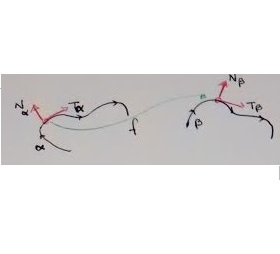
\includegraphics[width=0.4\textwidth]{C:/Users/Nacho/Documents/Latex/Facultad/GeometriaProyectiva/GeoProyectiva/teofundcurvasplanas.jpg}
	\caption{Un movimiento rígido que lleva un marco al otro.}
	\label{fig:teofundcurvasplanas}
\end{figure}


Consideremos la siguiente función: $$\Phi(s)=\norm{A_f\T_\alpha(s) - \T_\beta(s)}^2 + \norm{A_f\N_\alpha(s)-\N_\beta(s)}^2$$ Derivando el producto interno, obtenemos que: $$\Phi'(s)=2\pint{A_f\T_\alpha(s)-\T_\beta(s),A_f\T'_\alpha(s)-\T'_\beta(s)} + 2\pint{A_f\N_\alpha(s)-\N_\beta(s),A_f\N'_\alpha(s)-\N'_\beta(s)}$$ Notemos que $\T'_\alpha(s)= k(s)\N_\alpha(s)$ y $\N'_\alpha(s)=-k(s)\T_\alpha(s)$. En efecto, la primera es por definición de la curvatura plana. Por otra parte, como $\pint{\N_\alpha(s),\N'_\alpha(s)}=0$, tenemos que $\N'_\alpha(s)$ es paralelo a $\T_\alpha(s)$ y además derivando $\pint{\T_\alpha(s),\N_\alpha(s)}=0$ obtenemos que $\pint{\T'_\alpha(s),\N_\alpha(s)}+\pint{\T_\alpha(s),\N'_\alpha(s)} = 0$. Sabemos que el primer sumando es $k(s)$, y así se obtiene lo deseado. Distribuyendo las restas de los productos internos que aparecen en $\Phi'(s)$ y usando estas identidades, es fácil ver que $\Phi'(s)=0$. Es decir, $\Phi$ es constante.

Ahora bien, por cómo definimos el movimiento rígido, tenemos que $\Phi(s_0)=0$ (pues simplemente movimos el marco de una curva a la otra), y como $\Phi$ es constante, debe ser $\Phi(s)=0$. Como es una suma de cuadrados, ambos deben ser constantemente $0$ y así $0=A_f\T_\alpha(s)-\T_\beta(s) = (f\circ\alpha(s)-\beta(s))'$. Por lo tanto, $f\circ\alpha(s)-\beta(s)$ debe ser constante, y como $f\circ\alpha(s_0)=\beta(s_0)$, se sigue que $f\circ\alpha(s)=\beta(s)$ para todo $s\in I$. Es decir, construimos un movimiento rígido que lleva $\alpha$ a $\beta$. Y estamos.
\end{proof}
\end{teo}

\section{Curvas en el Espacio}

Ahora nos interesará estudiar curvas en el espacio $\sigma:I\to\RR^3$. Supongamos $\sigma$ parametrizada por longitud de arco. Ya no tenemos una forma canónica de completar al vector tangente $\T(s)$ a una base ortonormal como antes (pues necesitamos de dos vectores). Sin embargo, como $\norm{\T(s)}=1$, seguimos teniendo (al derivar el producto interno) que $\pint{\T(s),\T'(s)}=0$. En los puntos de curvatura no nula, podemos definir $\N(s)=\dfrac{\T'(s)}{\norm{\T'(s)}} = \dfrac{\T'(s)}{\kappa(s)}$ al \textbf{vector normal principal}. Geométricamente, se puede ver como la dirección en la que avanza la curva dentro del plano ortogonal a $\T(s)$. Ahora sí tenemos una forma canónica de completar a los vectores $\{\T(s),\N(s)\}$ a una base ortonormal orientada de $\RR^3$. Simplemente es el producto vectorial $\B(s)=\T(s)\wedge\N(s)$. El vector $\B(s)$ se denomina el \textbf{vector binormal}.  De esta manera, nos construímos un marco $\{\T(s),\N(s),\B(s)\}$ ortonormal orientado positivamente, que denominaremos el \textbf{triedro de Frenet-Serret}.

\begin{figure}[h]
	\centering
		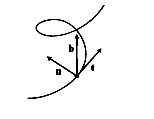
\includegraphics[width=0.4\textwidth]{C:/Users/Nacho/Documents/Latex/Facultad/GeometriaProyectiva/GeoProyectiva/frenetserret.jpg}
	\caption{El marco de Frenet-Serret.}
	\label{fig:frenetserret}
\end{figure}

\begin{defn}
Sea $\sigma:I\to\RR^3$ una curva regular parametrizada por longitud de arco. La \textbf{torsión} de la curva se define como $\tau(s)=-\pint{\B'(s),\N(s)}$.
\end{defn}

Antes de entender el por qué de la definición de la torsión y qué es lo que mide, veamos un ejemplo.

\begin{ex}
Consideremos la hélice circular de radio $r$ y velocidad vertical $b$, parametrizada por $\sigma(t) = (r\cos(\omega s),r\sen(\omega s),b\omega s)$ con $\omega = \dfrac{1}{\sqrt{r^2+b^2}}$, para que esté parametrizada por longitud de arco. Entonces $\T(s)=(-r\omega\sen(\omega s),r\omega\cos(\omega s),b\omega)$ y así tenemos que $\T'(s)=(-r\omega^2\cos(\omega s),-r\omega^2 \sen(\omega s),0)$. Por lo tanto, la curvatura de la hélice es $\kappa(s)=\norm{\T'(s)} = r\omega^2 = \dfrac{r}{r^2+b^2}$. Luego, el vector normal principal es $\N(s)=(-\cos(\omega s),\sen(\omega s),0)$. Calculando el producto vectorial, obtenemos que $\B(s)=\T(s)\wedge\N(s)=(b\omega\sen(\omega s),-b\omega\cos(\omega s),r\omega)$, y de esto se desprende que su derivada es $\B'(s)=(b\omega^2\cos(\omega s),b\omega^2 \sen(\omega s),0)$. Finalmente, la torsión debe ser $\tau(s)=-\pint{\B'(s),\N(s)} = b\omega^2 = \dfrac{b}{r^2+b^2}$.
\end{ex}

Estamos en condiciones de probar lo siguiente:

\begin{teo}[Frenet-Serret] Valen las siguientes ecuaciones: 
\begin{align*}\T' &=          & \kappa&\N &      & \\
              \N' &=-\kappa\T &           &      &+\tau\B \\ 
							\B' &=          &  -\tau&\N &      &\end{align*}
\begin{proof} Queremos expresar a $\{\T',\N',\B'\}$ en términos de la base ortonormal $\{\T,\N,\B\}$. La primera fórmula es obvia por la definición de $\N$.

Notemos que como $\pint{\T(s),\N(s)}=0$, derivando el producto interno tenemos que $\pint{\T'(s),\N(s)}+\pint{\T(s),\N'(s)}=0$. Como $\pint{\T'(s),\N(s)}=\pint{\kappa(s)\N(s),\N(s)}=\kappa(s)$, se sigue que $\pint{\T(s),\N'(s)}=-\kappa(s)$. Por otra parte, como $\norm{\N(s)}^2=1$, derivando el producto interno tenemos $\pint{\N(s),\N'(s)}=0$. Para calcular $\pint{\N'(s),\B(s)}$ simplemente notemos que $\pint{\N(s),\B(s)}=0$ y derivándolo tenemos $\pint{\N'(s),\B(s)}+\pint{\N(s),\B'(s)}=0$. Es decir, $\pint{\N'(s),\B(s)}=\tau(s)$. Como sabemos que $\{\T(s),\N(s),\B(s)\}$ es una base ortonormal, $\N'(s)=\pint{\N'(s),\T(s)}\T(s)+\pint{\N'(s),\N(s)}\N(s)+\pint{\N'(s),\B(s)}\B(s)$, y por lo que acabamos de calcular esto es $\N'(s) = -\kappa(s)\T(s) + \tau(s)\B(s)$.

Como tenemos $\B(s)=\T(s)\wedge\N(s)$, derivando el producto vectorial tenemos que $\B'(s)=\T'(s)\wedge \N(s) + \T(s)\wedge \N'(s)$. Ahora bien, $\T'(s)$ es paralelo a $\N(s)$ y así el producto vectorial entre ellos se anula $\T'(s)\wedge\N(s)=0$. Por otra parte, ya probamos la identidad $\N'(s)=-\kappa(s)\T(s)+\tau(s)\B(s)$ y así, distribuyendo el producto vectorial, obtenemos que $\B'(s)=\T(s)\wedge \N'(s)=-\kappa(s) \T(s)\wedge\T(s) + \tau(s) \T(s)\wedge\B(s) = -\tau(s)\N(s)$. Esto concluye la demostración.
\end{proof}
\end{teo}

La tercera fórmula de Frenet-Serret nos dice que la torsión mide precisamente cuánto la curva se está escapando del plano generado por $\{\T(s),\N(s)\}$, pues esto se puede ver como el cambio instantáneo en la dirección de la recta perpendicular al plano. Las fórmulas de Frenet-Serret nos dicen que $(\T,\N,\B)$ cumplen el siguiente sistema de ecuaciones diferenciales, que rigen el movimiento del marco a lo largo de la curva: $$\begin{pmatrix}\T' \\ \N'\\ \B'\end{pmatrix} = \begin{pmatrix}0& \kappa & 0 \\ -\kappa & 0 & \tau \\ 0 & -\tau & 0\end{pmatrix}\begin{pmatrix}\T \\ \N \\ \B\end{pmatrix}$$ Por el Teorema de Existencia y Unicidad para Ecuaciones Diferenciales Ordinarias, si le damos que el dato inicial sea el marco $(\T(s_0),\N(s_0),\B(s_0)) = (e_1,e_2,e_3)$ (pues cualquier marco es lo mismo ya que simplemente llevamos uno en otro con un movimiento rígido), obtenemos que hay una única solución al problema para $\kappa,\tau$ dadas. Es decir, la curvatura y la torsión nos van a determinar completamente a una curva en el espacio. Hagamos esto con mayor precisión:

\begin{teo}[Teorema Fundamental de las Curvas]
Sea $I=(a,b)$ un intervalo abierto no vacío y $\kappa,\tau:(a,b)\to\RR$ funciones tales que $\kappa\in\mathscr{C}^{k-2}(I),\tau\in\mathscr{C}^{k-3}(I)$ y $\kappa>0$. Entonces, existe una curva $\sigma:I\to\RR^3$ regular de clase $\mathscr{C}^k$ parametrizada por longitud de arco tal que $\kappa$ es la curvatura y $\tau$ la torsión de $\sigma$.
\begin{proof}
Consideremos el Problema de Valores Iniciales dado por: $$\begin{pmatrix}\T' \\ \N'\\ \B'\end{pmatrix} = \begin{pmatrix}0& \kappa & 0 \\ -\kappa & 0 & \tau \\ 0 & -\tau & 0\end{pmatrix}\begin{pmatrix}\T \\ \N \\ \B\end{pmatrix}$$ con dato inicial $(\T(s_0),\N(s_0),\B(s_0))=(e_1,e_2,e_3)$ para algún $s_0\in I$ fijo. Por el Teorema de Existencia y Unicidad, sabemos que hay una única solución $(\T,\N,\B):I\to(\RR^3)^3$. Veamos que para cada $s\in I$ se tiene que $\{\T(s),\N(s),\B(s)\}$ forma una base ortonormal. En efecto, para esto simplemente veamos que el producto interno de cada par de vectores del Triedro $\{\T(s),\N(s),\B(s)\}$ es constante. Como el dato inicial nos dice que forman una base ortonormal, al ser constantes, formarán en cada tiempo $s$ una base ortonormal. Para ello, consideremos la función $F:I\to\RR^6$ dada por $F(s)=\left(\norm{\T(s)}^2,\norm{\N(s)}^2,\norm{\B(s)}^2,\pint{\T(s),\N(s)},\pint{\N(s),\B(s)},\pint{\B(s),\T(s)}\right)$ y notemos que cumple el siguiente problema de valores iniciales: $$\begin{pmatrix}x_1'(s)\\ x_2'(s)\\x_3'(s)\\x_4'(s)\\x_5'(s)\\x_6'(s)\end{pmatrix} = \begin{pmatrix}0&0&0&2\kappa(s)&0&0\\ 0&0&0&-2\kappa(s)&2\tau(s)&0\\ 0&0&0&0&0&-2\tau(s)\\ -\kappa(s)&\kappa(s)&0&0&0&\tau(s)\\ 0&-\tau(s)&\tau(s)&0&0&-\kappa(s)\\0&0&0&-\tau(s)&\kappa(s)&0\end{pmatrix}\begin{pmatrix}x_1(s)\\ x_2(s)\\x_3(s)\\x_4(s)\\x_5(s)\\x_6(s)\end{pmatrix}$$ Con dato inicial $F(s_0)=(1,1,1,0,0,0)$ (simplemente es derivar los productos internos y usar que $\T',\N',\B'$ cumplen el sistema de ecuaciones diferenciales de Frenet-Serret). Ahora bien, notemos que la función $G(s)=(1,1,1,0,0,0)$ es una solución a ese Problema de Valores Iniciales. Eso implica que las normas deben ser constantemente $1$ y los productos internos constantemente $0$. Es decir, $\{\T(s),\N(s),\B(s)\}$ es una base ortonormal para todo $s\in I$. Más aún, está orientada positivamente, pues el signo de la orientación nos lo da el signo del determinante de la matriz cuyas columnas son $\{\T(s),\N(s),\B(s)\}$, que al ser una base ortonormal, es $1$ ó $-1$. Como el determinante depende continuamente de las entradas de la matriz, debe ser constantemente $1$ (pues $\{\T(s_0),\N(s_0),\B(s_0)\}$ está orientado positivamente), y así siempre tenemos la orientación correcta.

Consideremos la curva definida por $\sigma:I\to\RR^3$, $\sigma(s)=\displaystyle\int_{0}^s \T(\xi)\diff\xi$. Entonces $\sigma$ es de clase $\mathscr{C}^k$ y se cumple que $\sigma'(s)=\norm{\T(s)}=1$. Por lo tanto, $\sigma$ está parametrizada por longitud de arco. Como $\{\T(s),\N(s),\B(s)\}$ cumplen las ecuaciones de Frenet-Serret, es fácil ver que $\sigma$ tiene curvatura $\kappa$ y torsión $\tau$, pues es fácil ver que $\{\T(s),\N(s),\B(s)\}$ es el marco de Frenet-Serret asociado a $\sigma$.

Finalmente, supongamos que $\mu:I\to\RR^3$ es otra curva parametrizada por longitud de arco con curvatura $\kappa$ y torsión $\tau$. Sea $f:\RR^3\to\RR^3$ un movimiento rígido tal que $f(\sigma(s_0))=\mu(s_0)$ y lleva el triedro de $\mu$ en $s_0$, $\{\T_\mu(s_0),\N_\mu(s_0),\B_\mu(s_0)\}$ a la base ortonormal $\{\T(s_0),\N(s_0),\B(s_0)\}$ preservando la orientación. Ahora bien, como $A_f$ es una isometría directa y $\{\T_\mu(s),\N_\mu(s),\B_\mu(s)\}$ cumplen las ecuaciones de Frenet-Serret, debemos tener que $\{A_f\T_\mu(s),A_f\N_\mu(s),A_f\B_\mu(s)\}$ también las cumple y además tiene por dato inicial $(A_f\T_\mu(s_0),A_f\N_\mu(s_0),A_f\B_\mu(s_0))=(\T(s_0),\N(s_0),\B(s_0))$. Por la unicidad de la solución, tenemos que $A_f\T_\mu(s)=\T(s)$ para todo $s\in I$. Por lo tanto, concluimos que $(f\circ \mu(s) - \sigma(s))' = A_f\T_\mu(s)-\T(s) = 0$ y así $f\circ\mu(s)-\sigma(s)$ es constante. Como $f\circ\mu(s_0)=\sigma(s_0)$, se sigue que $f\circ\mu =\sigma$. Esto concluye la demostración.
\end{proof}
\end{teo}

Notemos que el triedro de Frenet-Serret nos determina, en cada punto de la curva, tres planos: el \textbf{plano osculador} es el plano ortogonal a $\B(s)$, el \textbf{plano normal} es el plano ortogonal a $\T(s)$ y el \textbf{plano rectificante} es el plano ortogonal a $\N(s)$. Tratemos de entender como son las proyecciones de la curva a cada uno de estos planos. Para esto, supongamos sin pérdida de la generalidad que $\sigma:(a,b)\to\RR^3$ está parametrizada por longitud de arco y $0\in (a,b)$, y estudiemos las proyecciones al triedro en $\sigma(0)$. Por el desarrollo en serie de Taylor, $\sigma(t)=\sigma(0)+\sigma'(0)t + \dfrac{\sigma''(0)}{2}t^2 + \dfrac{\sigma'''(0)}{6}t^3+ o(t^3)$ (donde usamos la notación $o$-chica, es decir $f(t)$ es $o(t^3)$ si $\displaystyle\lim_{t\to\infty}f(t)/t^3=0$). Por las ecuaciones de Frenet-Serret, sabemos que $\sigma'(0)=\T(0)$, $\sigma''(0)=\T'(0)=\kappa(0)\N(0)$ y finalmente $\sigma'''(0)=-\kappa^2(0)\T(0)+\kappa'(0)\N(0) + \kappa(0)\tau(0)\B(0)$. Como a menos de un movimiento rígido la curva es la misma, podemos suponer sin pérdida de la generalidad que $\sigma(0)=0$. Si escribimos todo en términos de la base $\{\T(0),\N(0),\B(0)\}$, obtenemos una aproximación de orden $3$ en un entorno del origen: $$\sigma(t)\approx\begin{pmatrix}1\\ 0\\ 0\end{pmatrix}t + \begin{pmatrix}0\\ \kappa(0)\\ 0\end{pmatrix}\dfrac{t^2}{2} + \begin{pmatrix}-\kappa(0)^2\\ \kappa'(0) \\ \kappa(0)\tau(0)\end{pmatrix}\dfrac{t^3}{6}$$
La proyección en el plano osculador, mirando los términos de orden $2$ sólamente, es una parábola parametrizada por $x(t)=t$, $z(t)=\dfrac{\kappa(0)}{2}t^2$. La proyección en el plano rectificante, mirando los términos de orden $3$ sólamente, es aproximadamente una cúbica parametrizada por $x(t)=t-\kappa(0)^2 t^3\approx t$, $y(t)=\dfrac{\kappa(0)\tau(0)}{6}t^3$. Finalmente, la proyección en el plano normal, mirando los términos de orden $3$ sólamente, es aproximadamente $y(t)\approx\dfrac{\kappa(0)}{2}t^2$, $z(t)=\dfrac{\kappa(0)\tau(0)}{6}t^3$.


\begin{figure}[h]
	\centering
		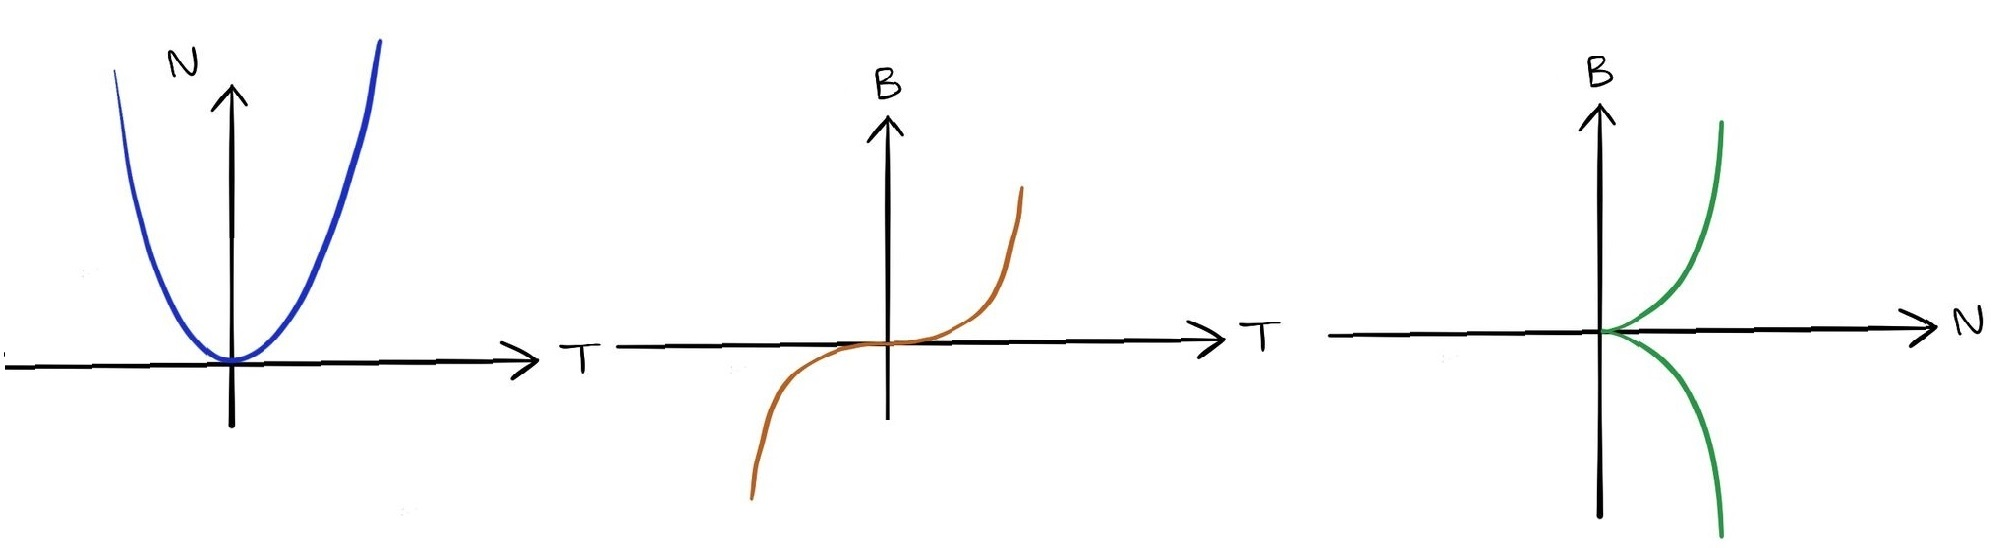
\includegraphics[width=1\textwidth]{C:/Users/Nacho/Documents/Latex/Facultad/GeometriaProyectiva/GeoProyectiva/proyeccionesfrenet.jpg}
	\caption{Las proyecciones a los planos que determina el Triedro de Frenet-Serret.}
	\label{fig:proyeccionesfrenet}
\end{figure}


\section{Resultados Globales}

Hemos probado que las curvas en el espacio están totalmente determinadas por su curvatura y torsión. Pero estos dos datos son locales. En un sentido más preciso, esto se debe a que se obtienen simplemente calculando derivadas en el punto y por la Observación ~\ref{obs::germenderivadas} ya sabemos que las derivadas son información local. En esta sección vamos a ver cómo obtener resultados globales a partir de información local. Veamos primero dos ejemplos sencillos.

\begin{prop}
Sea $\sigma:I\to\RR^3$ una curva tal que todas las rectas normales pasan por un punto $P\in\RR^3$ fijo. Entonces la imagen de $\sigma$ está contenida en una esfera.
\begin{proof}
Supongamos sin pérdida de la generalidad que $\sigma$ está parametrizada por longitud de arco. La recta normal a la curva en $\sigma(s)$ es la recta parametrizada por $L:\RR\to\RR^3$, $L(\lambda)=\sigma(s)+\lambda\N(s)$. Por lo tanto, para todo $s\in(a,b)$ existe un $\lambda(s)\in\RR$ tal que $P=\sigma(s)+\lambda(s)\N(s)$. Luego, tenemos que $\lambda(s) = \pint{P-\sigma(s),\N(s)}$, y así $\lambda$ es una función diferenciable. Derivando el producto interno, obtenemos que: $$\lambda'(s) = \pint{-\sigma'(s),\N(s)}+\pint{P-\sigma(s),\N'(s)} = -\pint{\T(s),\N(s)}+\pint{\lambda(s)\N(s),\N'(s)} = 0$$ Es decir, $\lambda$ es constante. Pero ahora, como $\lambda\N(s)=P-\sigma(s)$, tomando norma resulta que $\abs{\lambda} = \norm{P-\sigma(s)}$. Es decir, $\sigma$ está contenida en la circunferencia de centro $P\in\RR^3$ y radio $\abs{\lambda}$. Como queríamos probar.
\end{proof}
\end{prop}

\begin{prop}
Una curva en el espacio está contenida en un plano si y sólo si $\tau\equiv 0$.
\begin{proof}
\hfill

$(\Longleftarrow)$ Sea $\sigma:I\to\RR^3$ una parametrización por longitud de arco y $s_0\in I$. Por las ecuaciones de Frenet-Serret, $\B'(s)=-\tau(s)\N(s)=0$. Es decir, $\B$ es constante. Consideremos $\Pi$ el plano de ecuación $\pint{x-\sigma(s_0),\B}$. Veamos que $\sigma(s)\in\Pi$ para todo $s\in I$. En efecto, sabemos que $\sigma(s_0)\in\Pi$. Derivando el producto interno: $$\dfrac{\diff}{\diff s}\pint{\sigma(s)-\sigma(s_0),\B} = \pint{\T(s),\B} + \pint{\sigma(s)-\sigma(s_0),\B'} = 0$$ Por lo tanto, $\pint{\sigma(s)-\sigma(s_0),\B}$ debe ser constante y en $s_0$ es $0$. Como queríamos.

$(\Longrightarrow)$ Tenemos un movimiento rígido que lleva el plano que contiene a la curva al plano $xy$. Como la curvatura y la torsión son invariantes por movimientos rígidos, podemos asumir entonces que $\sigma:I\to\RR^3$ parametrizada por longitud de arco es de la forma $\sigma(s)=(x(s),y(s),0)$. Por lo tanto, $\T(s)=\sigma'(s)=(x'(s),y'(s),0)$, de donde obtenemos que la normal principal es $\N(s)=\dfrac{\T'(s)}{\kappa(s)}=\left(\dfrac{x''(s)}{\kappa(s)},\dfrac{y''(s)}{\kappa(s)},0\right)$, que es un vector unitario contenido en el plano $xy$. Es claro entonces que $\B(s) = (0,0,1)$ constantemente, pues es el producto vectorial entre dos vectores unitarios ortogonales contenidos en el plano $xy$. Esto implica que $\B'(s)=(0,0,0)$ y así la torsión debe ser nula. Y estamos.
\end{proof}
\end{prop}

\begin{defn}
Una curva $\sigma:\RR\to\RR^n$ regular se dice \textbf{cerrada} si existe $\rho>0$ tal que $\sigma(t+\rho)=\sigma(t)$ para todo $t\in\RR$. Al menor $\rho>0$ que cumple eso se lo denomina el \textbf{período}.
\end{defn}

\begin{obs}
Notar que el período existe. En efecto, si consideramos el conjunto: $$\mathscr{P}=\{\rho>0:\sigma(t+\rho)+\sigma(t)\;\forall t\in\RR\}$$ tomamos $\rho_0=\inf\mathscr{P}$, y $(\rho_n)_{n\in\NN}\subseteq\mathscr{P}$ una sucesión que tiende a $\rho_0$. Si tuviéramos que $\displaystyle\lim_{n\to\infty}\rho_n=0$, entonces $\sigma'(0)=\lim_{n\to\infty}\dfrac{\sigma(\rho_n)-\sigma(0)}{\rho_n} = 0$, que contradice la regularidad de $\sigma$. Por lo tanto $\rho_0>0$. Además, por la continuidad de $\sigma$, $\displaystyle\lim_{n\to\infty}\sigma(t+\rho_n)=\sigma(t+\rho_0)$, y así obtenemos $\sigma(t+\rho_0)=\sigma(t)$ para todo $t\in\RR$. Es decir, $\rho_0\in\mathscr{P}$ y así es un mínimo. Otra manera de verlo es notar que el conjunto $$\mathscr{S}=\{\rho\in\RR:\sigma(t+\rho)=\sigma(t)\;\forall t\in\RR\}$$ es un subgrupo del grupo aditivo $(\RR,+)$ y eso implica que es cíclico con un generador (sin pérdida de la generalidad positivo) que será el período, o que es denso, pero esto implicaría que $\sigma$ es constante.
\end{obs}

Notemos que la noción de longitud de una curva que tenemos, en el caso de una curva cerrada no refleja la situación geométrica. En efecto, la integral $\int_\RR \norm{\sigma'(\xi)}\diff\xi$ no será convergente nunca. Pero en realidad la información que nos importa está contenida en un período, y esto es lo que dice la siguiente definición:

\begin{defn}
Si $\sigma:\RR\to\RR^n$ es una curva cerrada, entonces se define la \textbf{longitud} de $\sigma$ como: $$\mathrm{Long}(\sigma)=\mathrm{Long}(\left.\sigma\right|_{[t,t+\rho]}) = \mathrm{Long}(\left.\sigma\right|_{[0,\rho]})$$
Una curva cerrada $\sigma$ de período $\rho$ se dice \textbf{simple} si $\sigma(t)=\sigma(s)$ implica $t-s\in\rho\ZZ$.
\end{defn}

Ya sabemos que la curvatura representa en alguna medida el cambio del ángulo de la curva en un sentido intuitivo, pero hasta ahora no formalizamos esta noción. Hagamos esto con la siguiente proposición:

\begin{prop}
\label{prop::anguloglobal}
Sea $\sigma:(a,b)\to\RR^2$ una curva regular plana y $k:(a,b)\to\RR$ su curvatura plana. Entonces existe una función $\theta:(a,b)\to\RR$ diferenciable tal que $$\T(s)=(\cos(\theta(s)),\sen(\theta(s)))$$ para todo $s\in(a,b)$. Se dice que $\theta$ es un \textbf{ángulo global}. Por otra parte, si $\varphi:(a,b)\to\RR$ es otro ángulo global, existe algún $\ell\in\ZZ$ tal que $\theta-\varphi\equiv 2\pi\ell$.
\begin{proof}
Supongamos primero que $\sigma$ está parametrizada por longitud de arco y sea $s_0\in(a,b)$. Como $\norm{\T(s_0)}=1$, existe $\theta_0\in\RR$ tal que $\T(s_0)=(\cos(\theta_0),\sen(\theta_0))$. Definamos una función $\theta:(a,b)\to\RR$ vía $\theta(t)=\theta_0 + \displaystyle\int_{t_0}^t k(\xi)\diff\xi$, y consideremos entonces $v:(a,b)\to\RR^2$ dada por $v(t)=(\cos(\theta(t)),\sen(\theta(t)))$. Si $R=\begin{pmatrix}0&-1\\1&0\end{pmatrix}\in\mathscr{M}_2(\RR)$, entonces es fácil verificar que $v'(t) = k(t)Rv(t)$. Pero por otra parte, $\T'(t)=k(t)R\T(t)$, y como $\T(t_0)=v(t_0)$, debemos tener que $\T\equiv v$ por la unicidad de la solución de este Problema de Valores Iniciales.

Ahora bien, si $\sigma$ no está parametrizada por longitud de arco, sea $u:(c,d)\to(a,b)$ la reparametrización tal que $\sigma\circ u$ sí esté parametrizada por longitud de arco. Entonces, existe un ángulo global $\theta:(c,d)\to\RR$ tal que $(\sigma\circ u)'(s)=(\cos(\theta(s)),\sin(\theta(s)))$. Por lo tanto, $\T(t)=\dfrac{\sigma'(t)}{\norm{\sigma'(t)}}=\sigma'(t)u'(u^{-1}(t)) = (\cos(\theta(u^{-1}(t))),\sen(\theta(u^{-1}(t))))$.

Por otra parte, si $\varphi$ es otro ángulo global, entonces tendremos que: $$(\cos(\theta(t)),\sen(\theta(t)))=\T(t)=(\cos(\varphi(t)),\sen(\varphi(t)))$$ y así $\theta(t)-\varphi(t)\in 2\pi\ZZ$. Como $\theta-\varphi$ es continua y $2\pi\ZZ$ es discreto, debe ser constante. Como queríamos probar.
\end{proof}
\begin{proof}[Una demostración topológica]
Sabemos que $p:\RR\to\mathrm{S}^1$, $p(t)=(\cos(t),\sen(t))$ es el revestimiento universal de $\mathrm{S}^1$. Sea $s_0\in(a,b)$ y $\theta_0\in\RR$ tal que $p(\theta_0)=\T(s_0)$. Como $(a,b)$ es simplemente conexo y $\T:(a,b)\to\mathrm{S}^1$ continua, por la propiedad del levantamiento, existe una única función continua $\theta:(a,b)\to\RR$ tal que $p\circ\theta=\T$ y $\theta(s_0)=\theta_0$. Es decir, el siguiente diagrama (de espacios topológicos punteados) conmuta:
\begin{center}
\begin{tikzcd}
& (\RR,\theta_0)\arrow[]{d}[font=\normalsize, right]{p} \\
((a,b),s_0)\arrow[dashed]{ur}[font=\normalsize]{\exists !\theta} \arrow[]{r}[font=\normalsize]{\T} & (\mathrm{S}^1,\T(s_0))
\end{tikzcd}
\end{center}
Ahora bien, como $p'(t)\neq 0$ para todo $t\in\RR$ y $p\in\mathscr{C}^\infty(\RR)$, por el Teorema de la Función Inversa existe en un entorno de cada punto una inversa infinitamente diferenciable $p^{-1}$ y así $\theta=p^{-1}\circ\T$ localmente. Por lo tanto, $\theta$ es tan diferenciable como $\T$, y listo.
\end{proof}
\end{prop}

\begin{defn}
Sea $\sigma:\RR\to\RR^2$ una curva cerrada de período $\rho$, y sea $\theta:(a,b)\to\RR$ un ángulo global para $\sigma$. Se define el \textbf{índice de rotación} de $\sigma$ como: $$\mathrm{Ind}(\sigma)=\dfrac{1}{2\pi}(\theta(\rho)-\theta(0))$$
\end{defn}

\begin{obs}
Notar que $\mathrm{Ind}(\sigma)$ no depende de la elección del ángulo global $\theta$ (pues si $\varphi$ es otro ángulo global, $\varphi(t)=\theta(t)+2\pi\ell$ y así $\varphi(\rho)-\varphi(0)=\theta(\rho)-\theta(0)$). Por otra parte, como $\sigma(\rho)=\sigma(0)$ por la periodicidad, obtenemos que $\theta(\rho)-\theta(0)\in 2\pi\ZZ$ y así $\mathrm{Ind}(\sigma)\in\ZZ$.
\end{obs}

\begin{teo}[Hopf]
\label{teo::hopfumlaufsatz}
El índice de rotación de una curva cerrada y simple es siempre $\pm 1$ (dependiendo de la dirección en la que se la parametriza).
\begin{proof}
Sea $\sigma:\RR\to\RR^2$ la curva parametrizada por longitud de arco con período $\rho$. Consideremos la región $\triangle = \{(s,t)\in\RR^2 : 0\leq s<t\leq \rho\}$, como en la Figura ~\ref{fig:hopfumlaufsatz1}

\begin{figure}[h]
	\centering
		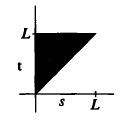
\includegraphics[width=0.3\textwidth]{C:/Users/Nacho/Documents/Latex/Facultad/GeometriaProyectiva/GeoProyectiva/hopfumlaufsatz1.jpg}
	\caption{La región $\triangle$.}
	\label{fig:hopfumlaufsatz1}
\end{figure}

Consideremos ahora la función $\varphi:\triangle\to\mathrm{S}^1\subseteq\RR^2$ dada por: $$\varphi(s,t)=\begin{cases}\dfrac{\sigma(t)-\sigma(s)}{\norm{\sigma(t)-\sigma(s)}} &\text{ si }0\leq s< t\leq \rho \text{ y } (s,t)\neq(0,\rho) \\ \T(s)=\sigma'(s) &\text{ si }0\leq s=t\leq\rho \\ -\T(0)=-\sigma'(0)&\text{ si }(s,t)=(0,\rho)\end{cases}$$

Es claro que esta función, asumiendo suficiente regularidad de $\sigma$, es al menos de clase $\mathscr{C}^2$ en $\triangle$ (es decir, hay un abierto que contiene a $\triangle$ y una función que extiende a $\varphi$ que es de clase $\mathscr{C}^2$). Como en la demostración topológica de ~\ref{prop::anguloglobal}, podemos conseguir una función $\theta:\triangle\to\RR$ diferenciable tal que $\varphi(s,t)=(\cos(\theta(s,t)),\sen(\theta(s,t)))$. Notemos que $\varphi(s,s)=\T(s)$ y así $\theta(s,s)$ es un ángulo global para $\sigma$. 

Como el índice de rotación claramente es invariante bajo movimientos rígidos y reparametrizaciones directas, podemos asumir que toda la imagen de $\sigma$ está contenida en el semiplano superior, de modo tal que $\sigma(0)=0$ y la tangente a $\sigma$ allí es paralela al eje $x$. Es decir, trasladamos la curva hasta que toque en su punto más bajo al eje $x$. Si su tangente tuviera alguna componente en la dirección del eje $y$, desarrollando en serie de Taylor en un entorno de ese punto, o bien vendría un punto desde abajo (si la componente fuera positiva) o bien iría hacia abajo (si la componente fuera negativa). Ambas alternativas serían contradictorias a que el punto sea el más bajo. Esto se puede observar en la Figura ~\ref{fig:hopfumlaufsatz2}

\begin{figure}[h]
	\centering
		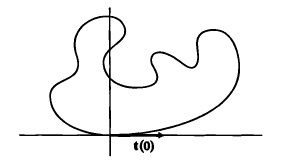
\includegraphics[width=0.55\textwidth]{C:/Users/Nacho/Documents/Latex/Facultad/GeometriaProyectiva/GeoProyectiva/hopfumlaufsatz2.jpg}
	\caption{Posicionando correctamente a la curva.}
	\label{fig:hopfumlaufsatz2}
\end{figure}

Supongamos que $\sigma$ se atraviesa de modo tal que $\T(0)=(1,0)$. Podemos parametrizar a los lados del triángulo $\triangle$ según $\gamma_1:[0,\rho]\to\RR^2,\;\gamma_1(t)=(0,t)$, $\gamma_2:[0,\rho]\to\RR^2$, $\gamma_2(t)=(t,\rho)$ y $\gamma:[0,\rho]\to\RR^2,\; \gamma(t)=(t,t)$. Como $\theta(s,s)$ es un ángulo global, se tiene claramente que: $$\mathrm{Ind}(\sigma)=\dfrac{1}{2\pi}(\theta(\rho,\rho)-\theta(0,0)) = \dfrac{1}{2\pi}\displaystyle\int_{0}^\rho \dfrac{\diff}{\diff u}(\theta(u,u))\diff u = \dfrac{1}{2\pi}\int_0^\rho \theta_s(u,u)+\theta_t(u,u)\diff u $$ Pero esta última integral simplemente es la integral de línea del campo $(\theta_s,\theta_t)$ sobre $\gamma$. Al ser $\theta$ de clase al menos $\mathscr{C}^2$, las derivadas cruzadas conmutan y esto implica que el campo es conservativo. Por lo tanto, la integral de línea depende solamente de los extremos y no del camino. Es decir, se tiene: $$\dfrac{1}{2\pi}\int_{\gamma} (\theta_s,\theta_t)\cdot \diff s = \dfrac{1}{2\pi}\int_{\gamma_1}(\theta_s,\theta_t)\cdot \diff s + \dfrac{1}{2\pi}\int_{\gamma_2}(\theta_s,\theta_t)\cdot\diff s$$
\textcolor{red}{COMPLETAR EL ARGUMENTO!}
\end{proof}
\end{teo}

\begin{cor}
Sea $\sigma:\RR\to\RR^2$ una curva cerrada simple. Entonces la función $\T:\RR\to\mathrm{S}^1$ es sobreyectiva.
\begin{proof}
Sea $\theta$ un ángulo global y $\rho$ el período de $\sigma$. Sin pérdida de la generalidad, por el Teorema anterior ~\ref{teo::hopfumlaufsatz}, tenemos $\theta(\rho)-\theta(0)=2\pi$. Por conexión, tenemos que $\theta$ debe tomar todos los valores en $[\theta(0),\theta(0)+2\pi]$. Esto implica que $\T$ es sobreyectiva, pues $\T(s)=(\cos(\theta(s)),\sen(\theta(s)))$ y $\theta$ recorre todo un período.
\end{proof}
\end{cor}

\begin{defn}
Una curva se dice \textbf{convexa} si está contenida a un lado de cada una de las rectas tangentes.
\end{defn}

\begin{teo}
Una curva cerrada simple es convexa si y sólo si su curvatura no cambia de signo.
\begin{proof}
\hfill

($\Longleftarrow$) Sea $\sigma:\RR\to\RR^2$ una parametrización por longitud de arco con período $\rho$, y sea $\theta:\RR\to\RR$ un ángulo global para $\sigma$. Entonces, sabemos que $\theta'=k$, y como la curvatura no cambia de signo, debemos tener que $\theta$ es monótona. Supongamos sin pérdida de la generalidad que $k\geq 0$ y así $\theta$ monótona creciente. Supongamos que $\sigma$ no es convexa. Es decir, existe un punto $p=\sigma(t_0)$ y puntos $q_1=\sigma(t_1),q_2=\sigma(t_2)$ en cada uno de los semiplanos que determina la tangente $L$ a $\sigma$ por $p$. Tomamos a $q_1$ y $q_2$ como los puntos más alejados de $L$. Claramente las rectas tangentes a $\sigma$ por $q_1$ y $q_2$ deben ser paralelas a $L$ pues si $\T(t_1),\T(t_2)$ tuvieran alguna componente en la dirección ortogonal a $L$, mirando el desarrollo de Taylor en un entorno de $s_1, s_2$ tendríamos puntos más alejados de $L$ (alternativamente, esto se puede probar por Multiplicadores de Lagrange).

\begin{figure}[h]
	\centering
		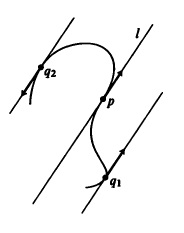
\includegraphics[width=0.30\textwidth]{C:/Users/Nacho/Documents/Latex/Facultad/GeometriaProyectiva/GeoProyectiva/curvaturacurvaconvexa.jpg}
	\caption{Los puntos más alejados a ambos lados de la tangente.}
	\label{fig:curvaturacurvaconvexa}
\end{figure}

Como tenemos tres vectores unitarios con la misma dirección, debe haber al menos dos que tengan el mismo sentido (y así deben ser idénticos). Es decir, tenemos $0\leq s_1<s_2\leq \rho$ tales que $\T(s_1)=\T(s_2)$ con $(s_1,s_2)\neq (0,\rho)$. Por lo tanto, $\theta(s_2)-\theta(s_1)\in 2\pi\ZZ$. Ahora bien, como $\theta$ es monótona, el incremento $\theta(s_2)-\theta(s_1)$ debe ser menor que $\theta(\rho)-\theta(0)$. Pero por el Teorema de Hopf ~\ref{teo::hopfumlaufsatz} debemos tener que $\theta(\rho)-\theta(0)=2\pi$. Entonces, $\theta(s_1)=\theta(s_2)$ ó $\theta(s_2)=\theta(s_1)+2\pi$. En el primer caso, $\theta$ debe ser constante en $[s_1,s_2]$ y así $\sigma$ debe ser una recta en $[s_1,s_2]$. Esto contradice el hecho de que ninguno de los puntos $p,q_1,q_2$ yacen sobre una misma recta. En el segundo caso, como $\theta(s_2)-\theta(s_1)=\theta(\rho)-\theta(0)$, debemos tener que $\theta$ es constante en $[0,s_1]$ y $[s_2,\rho]$. De esta forma, $\sigma$ es un segmento de recta entre $\sigma(s_1)$ y $\sigma(s_2)$, y esto es absurdo como en el caso anterior.

$(\Longrightarrow)$ Supongamos ahora que $\sigma$ es convexa. Si $\theta$ no es monótona, entonces existen $t_1<t_0<t_2$ tales que $\theta(t_1)=\theta(t_2)$ pero $\theta(t_1)\neq\theta(t_0)$. \textcolor{red}{Agregar una justificación decente para esto}. En particular tenemos que $\T(t_1)=\T(t_2)$.

Como $\T$ es sobreyectiva, existe $t_3$ tal que $\T(t_3)=-\T(t_1)$. Si miro las rectas tangentes a $\sigma$ en tiempos $t_1,t_2,t_3$, tengo tres rectas paralelas con puntos de la curva. Si tomo la que está en el medio, tiene puntos a ambos lados y eso niega la convexidad de la curva. Por lo tanto, al menos dos de esas rectas tangentes deben coincidir. Supongamos que $\sigma(s_1)$ y $\sigma(s_2)$ tienen la misma recta tangente $L$. Sea $L'$ una recta perpendicular a $L$ que corta a $L$ entre $\sigma(s_1)$ y $\sigma(s_2)$. Entonces, $L'$ debe cortar a la curva en dos puntos $p,q$, pues hay dos arcos de la curva entre $\sigma(s_1)$ y $\sigma(s_2)$. Supongamos que $p$ es el punto más cercano a $L$ y $q$ el más lejano de los dos. Si $p$ no está sobre $L$, entonces tenemos un triángulo con vértices $\sigma(s_1),\sigma(s_2)$ y $q$ con un punto $p$ en su interior. Ahora, cualquier recta que pase por $p$ no puede tener a $\sigma(s_1),\sigma(s_2)$ y $q$ en un mismo semiplano. En efecto, esto se debe a que los semiplanos son convexos y si tuviera a los tres vértices debería tener a todo el triángulo. En particular, $p$ estaría en el interior del semiplano y no en el borde. En particular, la tangente por $p$ nos dejaría puntos a ambos lados, lo que contradice la convexidad de $\sigma$. Esto implica que la curva tiene un segmento de recta entre $\sigma(s_1)$ y $\sigma(s_2)$.

\begin{figure}[h]
	\centering
		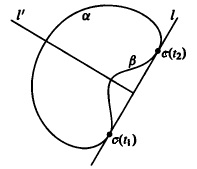
\includegraphics[width=0.30\textwidth]{C:/Users/Nacho/Documents/Latex/Facultad/GeometriaProyectiva/GeoProyectiva/tangentecurvaconvexa.jpg}
	\caption{Dos puntos en la curva con la misma recta tangente.}
	\label{fig:tangentecurvaconvexa}
\end{figure}

Esto es absurdo, pues la tangente en $s_1$ y $s_2$ tienen la misma dirección pero signo opuesto, y en todo ese segmento la tangente preserva la dirección, pero por continuidad no puede cambiar su signo. Este absurdo viene de suponer que $\theta$ no es monótona. Esto concluye la demostración.
\end{proof}
\end{teo}

\begin{cor}
Si $\sigma:\RR\to\RR^2$ es una curva cerrada, simple y convexa y $\theta(s_1)=\theta(s_2)$ ($s_1<s_2$) para algún ángulo global $\theta$, entonces $\theta$ es constante en $[s_1,s_2]$.
\begin{proof}
Se desprende de la demostración anterior.
\end{proof}
\end{cor}

\begin{cor}\label{cor::intconvrecta}
Sea $\sigma:\RR\to\RR^2$ una curva cerrada convexa. Si una recta interseca a $\sigma$ tres veces, entonces la interseca en todo el segmento entre esos dos puntos.
\begin{proof}
Supongamos que la recta $L$ corta a $\sigma$ en puntos $A,B,C$ con $B$ entre $A$ y $C$ en $L$. Notemos que $L$ debe ser tangente a $\sigma$ en $B$ pues si no $A$ y $C$ estarían en dos semiplanos distintos respecto de la tangente, lo que contradiría la convexidad de la curva. Pero entonces $L$ también debe ser tangente a la curva en $A$ y $C$, pues si la tangente a $\sigma$ en esos puntos tuviera alguna componente en la dirección ortogonal a $L$, habría puntos de la curva a ambos lados de $L$ (razonando como ya lo hicimos antes, por Taylor). Pero por el Corolario anterior, la curva debe ser una recta entre $A$ y $B$ y entre $B$ y $C$. Esto concluye la demostración.
\end{proof}
\end{cor}

\begin{defn}
Un \textbf{vértice} de una curva regular $\sigma:I\to\RR^2$ es un punto $s_0$ tal que $k'(s_0)=0$, donde $k$ es la curvatura plana de $\sigma$.
\end{defn}

\begin{teo}[de los Cuatro Vértices]
Sea $\sigma:\RR\to\RR^2$ una curva simple, cerrada y estrictamente convexa. Entonces $\sigma$ tiene al menos cuatro vértices.
\begin{proof}
Si $k$ fuera constante en algún intervalo, todos esos puntos serían vértices y el Teorema se seguiría trivialmente. Si $\rho$ es el período de $\sigma$, como $k:[0,\rho]\to\RR$ es una función continua sobre un compacto, alcanza un máximo y un mínimo en puntos $s_1,s_2$ respectivamente. Sean $p=\sigma(s_1)$ y $q=\sigma(s_2)$, y sea $L$ la recta que pasa por $p$ y $q$. Estos puntos $p$ y $q$ son claramente vértices por cómo los elegimos. Además, en virtud del Corolario ~\ref{cor::intconvrecta}, $L$ sólo puede cortar a la curva en $p$ y $q$. Sean $a,c\in\RR^2$ tales que la recta $L$ tiene ecuación $L=\{x\in\RR^2 : \pint{x-a,c}=0\}$. Entonces, la asignación $t\mapsto\pint{\sigma(t)-a,c}$ tiene exactamente dos ceros, que son $s_1$ y $s_2$. Veamos que en cada uno de dos los arcos de la curva que determinan $p$ y $q$ hay algún vértice. Esto nos dará los cuatro vértices que buscamos.

\begin{figure}[h]
	\centering
		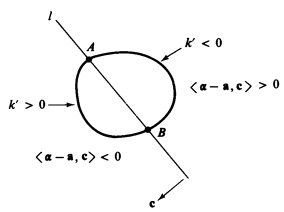
\includegraphics[width=0.40\textwidth]{C:/Users/Nacho/Documents/Latex/Facultad/GeometriaProyectiva/GeoProyectiva/fourvertex.jpg}
	\caption{El máximo y el mínimo de la curvatura de $\sigma$.}
	\label{fig:fourvertex}
\end{figure}

Integrando por partes, resulta que: \begin{align*}\int_{0}^{\rho} k'(t)\pint{\sigma(t)-a,c}\diff t &= -\int_{0}^{\rho}k(t)\pint{\T(t),c}\diff t + \left(k(t)\pint{\sigma(t)-a,c}\right)\Big\rvert_{0}^{\rho}\\ &= \int_{0}^{\rho} \pint{-k(t)\T(t),c}\diff t\\ &= \int_{0}^{\rho}\pint{\N'(t),c}\diff t\\ &=\int_{0}^{\rho}\pint{\N(t),c}'\diff t = \pint{\N(t),c}\Big\rvert_{0}^{\rho} = 0 \end{align*}

Ahora bien, en cada uno de los arcos de la curva que determinan $p$ y $q$, la derivada de la curvatura no se anula. Como $p$ es un mínimo y $q$ un máximo, en un arco la derivada de la curvatura debe ser positiva y en el otro negativa. Como la curva es convexa y estamos asumiendo que no hay un segmento contenida, hay un arco contenido en cada semiplano que determina $L$. En el semiplano que está por debajo de $L$ tendremos que $\pint{\sigma(t)-a,c}<0$ y en el que está por arriba tendremos que $\pint{\sigma(t)-a,c}>0$. Por lo tanto, $k'(t)\pint{\sigma(t)-a,c}$ siempre tiene el mismo signo en toda la curva. Pero probamos que $\displaystyle\int_{0}^{\rho}k'(t)\pint{\sigma(t)-a,c}\diff t=0$, y eso implica que $k'(t)\pint{\sigma(t)-a,c}\equiv 0$. Pero esto es absurdo, pues $\pint{\sigma(t)-a,c}$ se anula únicamente en $s_1$ y $s_2$, y estamos suponiendo que $k'$ se anula sólo en $s_1$ y $s_2$. Y estamos.
\end{proof}
\end{teo}
